%% ----------------------------------------------------------------
%% Thesis.tex -- MAIN FILE (the one that you compile with LaTeX)
%% ---------------------------------------------------------------- 

% Set up the document
\documentclass[a4paper, 11pt, oneside]{Thesis} % Use the "Thesis" style, based on the ECS Thesis style by Steve Gunn
\graphicspath{Figures/} % Location of the graphics files (set up for graphics to be in PDF format)

\usepackage{graphicx}
\usepackage{caption}
%\usepackage{subcaption}
\usepackage{float}

\usepackage[utf8]{inputenc}    % utf8 support   
\usepackage[T1]{fontenc}       % code for pdf file 
\usepackage{microtype}
% Include any extra LaTeX packages required
\usepackage[style=nature]{biblatex}
\addbibresource{Bibliography.bib}

%\usepackage[square, numbers, comma, sort&compress]{natbib} % Use the "Natbib" style for the references in the Bibliography
\usepackage{verbatim} % Needed for the "comment" environment to make LaTeX comments
\usepackage{vector} % Allows "\bvec{}" and "\buvec{}" for "blackboard" style bold vectors in maths
\hypersetup{urlcolor=blue, colorlinks=true} % Colours hyperlinks in blue, but this can be distracting if there are many links.
\usepackage{amsmath}
\usepackage{ dsfont }
\usepackage[inline]{enumitem}
\usepackage[table,xcdraw]{xcolor}
\usepackage{amssymb}
\usepackage{todonotes}
\usepackage{multirow}
\usepackage{diagbox}
\usepackage{soul}
\usepackage{commath}


\usepackage{tabularx,booktabs}
\newcolumntype{Y}{>{\centering\arraybackslash}X}

%%%%%%%%%%%%%%%%%%%%%%

\usepackage{algorithm}
\usepackage[noend]{algpseudocode}

\makeatletter
\def\BState{\State\hskip-\ALG@thistlm}
\makeatother

%%%%%%%%%%%%%%%%%%

% test
\usepackage{tikz}
\usetikzlibrary{shapes.geometric, arrows, chains, calc}
\usetikzlibrary{arrows.meta}

\usepackage{mathtools}  % amsmath with extensions
\usepackage{amsfonts}  % (otherwise \mathbb does nothing)
\def\realnumbers{\mathbb{R}}

\DeclareMathOperator{\E}{\mathbb{E}}
\DeclareMathOperator*{\argmin}{arg\,min} % thin space, limits underneath in displays
\DeclareMathOperator*{\argmax}{arg\,max} % thin space, limits underneath in displays

%% ----------------------------------------------------------------
\begin{document}

\frontmatter  % Begin Roman style (i, ii, iii, iv...) page numbering

% Set up the Title Page
\title {Reinforcement Learning for Robotic Actors in Multi-Agent Setups}
\authors {\texorpdfstring
  {\href{yoann.ponti@gmail.com}{Yoann Ponti}}
  {Yoann Ponti}
  }
\addresses {\groupname\\\deptname\\\univname} % Do not change this here, instead these must be set in the "Thesis.cls" file, please look through it instead
\date  {\today}
\subject {}
\keywords {}

\maketitle
%% ----------------------------------------------------------------

\setstretch{1.3} % It is better to have smaller font and larger line spacing than the other way round

% Define the page headers using the FancyHdr package and set up for one-sided printing
\fancyhead{} % Clears all page headers and footers
\rhead{\thepage} % Sets the right side header to show the page number
\lhead{} % Clears the left side page header

\pagestyle{fancy} % Finally, use the "fancy" page style to implement the FancyHdr headers

% %% ----------------------------------------------------------------
% % Declaration Page required for the Thesis, your institution may give you a different text to place here
% \Declaration{

% \addtocontents{toc}{\vspace{1em}} % Add a gap in the Contents, for aesthetics

% I, AUTHOR NAME, declare that this thesis titled, `THESIS TITLE' and the work presented in it are my own. I confirm that:

% \begin{itemize} 
% \item[\tiny{$\blacksquare$}] This work was done wholly or mainly while in candidature for a research degree at this University.
 
% \item[\tiny{$\blacksquare$}] Where any part of this thesis has previously been submitted for a degree or any other qualification at this University or any other institution, this has been clearly stated.
 
% \item[\tiny{$\blacksquare$}] Where I have consulted the published work of others, this is always clearly attributed.
 
% \item[\tiny{$\blacksquare$}] Where I have quoted from the work of others, the source is always given. With the exception of such quotations, this thesis is entirely my own work.
 
% \item[\tiny{$\blacksquare$}] I have acknowledged all main sources of help.
 
% \item[\tiny{$\blacksquare$}] Where the thesis is based on work done by myself jointly with others, I have made clear exactly what was done by others and what I have contributed myself.
% \\
% \end{itemize}
 
 
% Signed:\\
% \rule[1em]{25em}{0.5pt} % This prints a line for the signature
 
% Date:\\
% \rule[1em]{25em}{0.5pt} % This prints a line to write the date
% }
% \clearpage % Declaration ended, now start a new page

% % ----------------------------------------------------------------
% % The "Funny Quote Page"
% \pagestyle{empty} % No headers or footers for the following pages

% \null\vfill
% % Now comes the "Funny Quote", written in italics
% \textit{``Write a funny quote here.''}

% \begin{flushright}
% If the quote is taken from someone, their name goes here
% \end{flushright}

% \vfill\vfill\vfill\vfill\vfill\vfill\null
% \clearpage % Funny Quote page ended, start a new page
% % ----------------------------------------------------------------

% The Abstract Page
\addtotoc{Abstract} % Add the "Abstract" page entry to the Contents
\abstract{
\addtocontents{toc}{\vspace{1em}} % Add a gap in the Contents, for aesthetics


This exploratory work looks at a decentralised multi-agent reinforcement learning problem in which each agent is trying to maximise a global utility. Agents having only access to partial observations of the environment, a key challenge is coordination. To mitigate the effect of the partial observability, the agents must learn to communicate and share the information required to solve the task. The main objective of this work is to provide an in-depth look at the quality of the learning, the behaviour of the agents and the learned communication protocols. 
    
    


}

\clearpage % Abstract ended, start a new page
%% ----------------------------------------------------------------

\setstretch{1.3} % Reset the line-spacing to 1.3 for body text (if it has changed)

% The Acknowledgements page, for thanking everyone
\acknowledgements{
\addtocontents{toc}{\vspace{1em}} 

First and foremost, I would like to thank my supervisor Mischa Schmidt Ph.D. as well as S\'ebastien Nicolas and Anett Schuelke  Ph.D. for providing guidance and encouragement in carrying out this project at NEC Laboratories Europe GmbH. I respect and thank Prof. Boi Faltings for agreeing to supervise me and give me the opportunity to do a project in the industry. My thanks and appreciations also go to my colleagues in developing the project and people who have willingly helped me out with their abilities. I would like to particularly thank, Julia G., Cristof K., Shahd S. and Mauricio F. A. for their thorough proofreading and feed backs.

}
\clearpage % End of the Acknowledgements
%% ----------------------------------------------------------------

\pagestyle{fancy} %The page style headers have been "empty" all this time, now use the "fancy" headers as defined before to bring them back


%% ----------------------------------------------------------------
\lhead{\emph{Contents}} % Set the left side page header to "Contents"
\tableofcontents % Write out the Table of Contents

%% ----------------------------------------------------------------
\lhead{\emph{List of Figures}} % Set the left side page header to "List if Figures"
\listoffigures % Write out the List of Figures

%% ----------------------------------------------------------------
\lhead{\emph{List of Tables}} % Set the left side page header to "List of Tables"
\listoftables % Write out the List of Tables

%% ----------------------------------------------------------------
\setstretch{1.5} % Set the line spacing to 1.5, this makes the following tables easier to read
\clearpage % Start a new page
\lhead{\emph{Abbreviations}}  % Set the left side page header to "Abbreviations"
\listofsymbols{ll}  % Include a list of Abbreviations (a table of two columns)
{
\textbf{AI} & \textbf{A}rtificial \textbf{I}ntelligence \\
\textbf{Dec-POMDP} &  \textbf{D}ecentralised \textbf{P}artially \textbf{O}bservable \textbf{M}arkov \textbf{D}ecision \textbf{P}rocess \\
\textbf{MARL} & \textbf{M}ulti-\textbf{A}gent \textbf{R}einforcement \textbf{L}earning \\
\textbf{MAS}  & \textbf{M}ulti-\textbf{A}gent \textbf{S}ystem \\
\textbf{MC} & \textbf{M}onte-\textbf{C}arlo\\
\textbf{MDP} & \textbf{M}arkov \textbf{D}ecision \textbf{P}rocess \\
\textbf{POMDP} &  \textbf{P}artially \textbf{O}bservable \textbf{M}arkov \textbf{D}ecision \textbf{P}rocess \\
\textbf{RL} & \textbf{R}einforcement \textbf{L}earning \\ 
\textbf{ROS} & \textbf{R}obot \textbf{O}perating \textbf{S}ystem \\
\textbf{TD} & \textbf{T}emporal \textbf{D}ifference \\ 
} % Introduction

%% ----------------------------------------------------------------
% \clearpage % Start a new page
% \lhead{\emph{Physical Constants}} % Set the left side page header to "Physical Constants"
% \listofconstants{lrcl} % Include a list of Physical Constants (a four column table)
% {
% % Constant Name & Symbol & = & Constant Value (with units) \\
% Speed of Light & $c$ & $=$ & $2.997\ 924\ 58\times10^{8}\ \mbox{ms}^{-\mbox{s}}$ (exact)\\

% }

%% ----------------------------------------------------------------
\clearpage %Start a new page
\lhead{\emph{Symbols \footnote{The nomenclature put in place in \cite{sutton_reinforcement_1998} is used.}}}  % Set the left side page header to "Symbols"

\listofnomenclature{lll}  % Include a list of Symbols (a three column table)
{
$\alpha$, $\beta$ & step-size parameters\\
$\gamma$ & discount-rate factor \\
% symbol & name & unit \\
$s$ & a state &  \\
$a$ & an action &  \\
$r$ & a reward &  \\
$o$ & an observation (related to a state $s$)\\
$v$ & communication symbol \\
$A$ & set of available actions \\
$S$ & set of states \\
$O$ & set of observations\\
$V$ & set of communication symbols (vocabulary) \\

$t$ & discrete time step \\
$T$ & final time step of an episode \\
$G_t$ & return following time t \\
$\pi$ & policy \\
$\pi^*$ & optimal policy \\
$\pi(s)$ & action taken in state $s$ under deterministic policy $\pi$ \\
$\pi(a|s)$ & probability of taking action $a$ in state $s$ under stochastic policy $\pi$ \\

$v_{\pi}(s)$ & value of state $s$ under policy $\pi$ (expected return)\\
$v_{\pi^*}(s)$ & value of state $s$ under the optimal policy\\
$q_{\pi}(s, a)$ & value of taking action $a$ in state $s$ under policy $\pi$ \\
$q_{\pi^*}(s, a)$ & value of taking action $a$ in state $s$ under optimal policy\\

$V$ & array estimates of state-value function $v_{\pi}$ \\
$Q$ & array estimates of action-value function $q_{\pi}$\\
}
%% ----------------------------------------------------------------
% End of the pre-able, contents and lists of things
% Begin the Dedication page

\setstretch{1.3} % Return the line spacing back to 1.3

\pagestyle{empty} % Page style needs to be empty for this page

\dedicatory{}

\addtocontents{toc}{\vspace{2em}} % Add a gap in the Contents, for aesthetics


% ----------------------------------------------------------------
\mainmatter	 % Begin normal, numeric (1,2,3...) page numbering
\pagestyle{fancy} % Return the page headers back to the "fancy" style

% Include the chapters of the thesis, as separate files
% Just uncomment the lines as you write the chapters

\chapter{Introduction}
\lhead{\emph{Introduction}} 
Reinforcement learning has seen a lot of improvement since its first introduction and it has now been used to help solve many tasks thought before as unsolvable. For example, reinforcement learning has been used to beat human players at Atari games \cite{mnih_playing_2013} or master the game of GO \cite{silver_mastering_2016}. Moreover, reinforcement learning by solving the task of sequential decision making in an unknown environment is particularly well suited to solve tasks where it is difficult to obtain training data (robotics, telecommunication, etc.). 

% http://www.scholarpedia.org/article/Reinforcement_learning#Challenges_and_extensions_to_RL

Despite the usefulness of reinforcement learning in many fields, the method can lead to several problems. In an ideal world, any machine learning method should be able to cope with noisy input. Moreover, it should be general enough and scalable. In order to be able to learn, an agent requires feedback about the quality of the action taken. Unfortunately in most of the real-world scenarios, the feedback might be temporally delayed and as a result only impact the preceding states and actions weakly. For example, a robot might have to take several actions before relevant events happen. Several reinforcement learning algorithms assume the environment to be Markovian and that it is irrelevant how it has reached a certain state. Reinforcement learning agents might not know exactly in what state they are or will be after performing an action. Consequently, the preceding assumption is broken. Finally, reinforcement learning can only cope with dynamics that change slowly. This is a fundamental problem. Convergence of the learning might not be achievable if the world changes too fast \cite{kaelbling_reinforcement_1996}. Setting up a reinforcement learning problem might reveal itself to be difficult. Whether it is a real-world problem or a simulated one, appropriate state and action spaces need to be determined. In order to cover all possible situations, the state space as well as the available actions might be large. Exploring all possible pairs can then lead to a combinatorial explosion \cite{busoniu_comprehensive_2008, busoniu_multi-agent_2010}. The situation worsens when multiple agents are involved. The problem becomes exponential in the number of agents \cite{l._leottau_decentralized_2017}.

In order to cope with the curse of dimensionality, several solutions have been proposed such as generalising value functions. This is either done using function approximation methods or by interpolation of the searchable value-space. When the "action dimensions are able to operate in parallel and their individual information and resources can be managed separately", the task can be decentralised \cite{l._leottau_decentralized_2017}. It has been shown that decentralised systems are able to achieve similar learning times and comparable or slightly lower performance. To compensate the lack of direct coordination between the agents which can lead to lower performance, inter-agent communication can be used. Communication can help increase the team performance by mitigating two sources of uncertainty. It can help agents by increasing their knowledge about the state of the system as well as the intention of the other agents \cite{t._j._spaan_decentralized_2006}. The following explores this specific approach in a robotic transport system. In particular, the usage of the learned communication protocols is examined in-depth. 

\section{Contributions}

This Master project explores the application of distributed reinforcement learning in a coordination problem involving robotic arms. It explores inter-agent communication in a $Dec$-$POMDP$ environment to enable learning in a fully decentralised fashion. The communication protocols are also examined in order to to gain insight in the influence of the hyperparameters on the solutions. 

\section{Limits}

In order to study the behaviour of the agents, several assumptions had to be made. Even though the underlying problem is linked to the physical world, only simulated experiments are used. The problem is sufficiently simple to obtain good understanding of the underlying process and know which state information is relevant. This might not always be possible. This work relies on tabular Q-Learning. It enables faster learning and a clear view of the learning process. Unfortunately, this learning algorithm does not scale to more complex problems. Also the simulated environment makes assumption about the available interaction between the entities. The simulated environment look pass many problems that could arise in a real-world setting.

\section{Outline}
The work is organised as follows. In \autoref{chap:background}, the theoretical background linked to reinforcement learning and the Markov decision process framework are introduced. Furthermore, the necessary extensions needed by the transition from single agent to a multi-agent system as well as the related works are presented. The \autoref{chap:experiments} presents the experiment setting used in \autoref{chap:discussion}. The latter presents, examines and discusses the results. In particular this chapter describes the influence of hyperparameters on the quality of the learned communication. Finally, \autoref{chap:conclusion} discusses future work and concludes. % Introduction
\chapter{Background}
\lhead{\emph{Background}} 
\label{chap:background}	

The goal of machine learning is to avoid solving a specific task by explicitly programming an algorithm. In order to do this, machine learning tries to optimise a performance criterion using example data or past experience. When trying to solve a new task, it might be difficult to design a complete specification of the algorithm behaviour while it might be possible to obtain samples of the expected behaviour or to get feedback on the quality of the behaviour. Machine learning models can be predictive, i.e. make predictions based on new data, or descriptive, when the task of the model is to gain knowledge from data, or both \cite{alpaydin_introduction_2010}.

Reinforcement learning can be loosely related to how we as humans, learn to interact with our environment. For most of our life we do not have access to an explicit teacher, but we do have access to a direct sensorimotor connection to our environment providing feedback. Leveraging this feedback offers an indication about the consequences of an interaction with the environment. This indication can help us determine what to do to achieve a certain outcome. Reinforcement learning is the machine learning approach for learning goal oriented tasks from interaction.

Other approaches to machine learning include \textit{supervised learning} and \textit{unsupervised learning}. In supervised learning, a set of labelled examples provided by an external entity is used for the learning. Although supervised learning has been shown to be highly efficient for certain problems, obtaining the input-output pairs in an interactive problem can be extremely difficult. Indeed, the pairs should be representative of the expected behaviour as well as of all the states in which the agent should act. On the other hand, unsupervised learning finds hidden relationships between unlabelled inputs. Despite reinforcement learning having no direct access to the input-output examples, it should be considered a paradigm in its own right and not a kind of unsupervised learning. Indeed, it tries to maximise a reward signal instead of finding hidden pattern in the inputs.

Instead of relying on an oracle to instruct a learner the best action to take, reinforcement learning has to rely on a signal related to the quality of its decision \cite[p.~25]{sutton_reinforcement_1998}. The signal, which indicates what to do, but not how to do it, is expressed by a sanction called a \textit{reward} \cite[p.~18]{yves_glorennec_reinforcement_2001}. The reward can be positive, negative or neutral. It might be influenced by the taken action as well as the agent's past actions (delayed impact). The goal of reinforcement learning is thus to optimise a reward function by interacting with its environment (i.e. taking actions) and observing the resulting reward \cite{g._barto_1_2008}. Actions which have a positive outcome or avoid negative one will be preferred (reinforced). This is why reinforcement learning can be seen as a trial and error search.

% - learning agent must have access to: information about the current state, mean to affect the environment through interaction, and an indication about the quality of the interaction

% - RL is a sort of trial and error search
% - Use training information which evaluates action rather than instructs by giving correct action [RLNA p.25]
% - require reward, i.e. indication of the quality of interaction, because no oracle exists
% - Oracle could indicate which is the best action to take in this situation.
% - can see reward as a sanction (positive, neg or neutral) [RLAO p18] which indicates what to do but not how to do it
 
% - Must be able to take into account the fact that an action might have a direct or indirect (delayed) impact on following reward
% - optimizing an unknown reward function without direct access to the function but with the ability of taking actions observing the resulting reward. [Reinforcement learning and its relationship with supervise learning Andrew G barot]
% - agent needs to balance between exploration and exploitation to avoid getting stuck in local optima [EDMALAS Tuyls]

% - Action which have a positive return will be favoured over time, i.e the benefice behaviour will be reinforced. 
% => trade -off of exploration and exploitation.

\section{Markov Decision Processes}

In reinforcement learning, it is important to make the distinction between an agent and the environment. An agent is a computational mechanism able to learn and to take actions based on external information \cite{panait_cooperative_2005}. The environment is everything else. More precisely, it is everything which cannot directly be modified by the agent \cite[p.~50]{sutton_reinforcement_1998}.

\begin{figure}
\centering
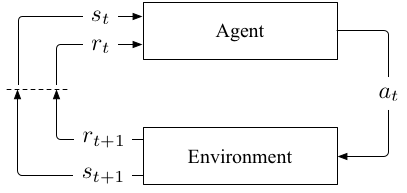
\includegraphics[width=0.5\textwidth]{imgs/rl-env.png}
\caption[The agent-environment interactions in a Markov decision process]{The agent-environment interactions in a Markov decision process \protect\footnotemark.}
\label{fig:agent-env-interaction}
\end{figure}


\footnotetext{Figure taken from \cite{sutton_reinforcement_1998}.}


The interaction between an agent and the environment is done at discrete time-steps. At each time-step, the agent observes the environment and takes an action accordingly. The environment will then transition to another state and provide a numerical signal, the reward, related to the transition. When a single agent is present in the environment, Markov decision processes (MDPs) can be leveraged to express mathematically the reinforcement learning problem \cite{puterman_markov_1995}. The interaction of the agent with the environment as depicted in fig.~\ref{fig:agent-env-interaction} creates a sequence of tuples $(s_t, a_t, r_t, s_{t+1})$ describing one \textit{trajectory} or \textit{episode}. Besides a finite set of states and actions, $S$ and $A$, the MDP requires a definition of its dynamics. The dynamics of any MDP can be defined by the probability to move to state $s' \in S$ and receive reward $r \in \realnumbers$ by taking action $a \in A$ in state $s \in S$.

$$p(s', r | s, a) = P(s_{t}=s', r_{t}=r \mid s_{t-1}=s, a_{t-1}=a)$$

Based on the recorded trajectory, it is possible to calculate the return or the sum of reward from time $t$ to the end of the episode.

$$G_t=\sum_{k=0}^{T} \gamma^{k} r_{t+k+1} = r_{t+1} + \gamma G_{t+1} \text{ with } G_T=0$$

Because an episode can be infinite (continuing task) or finite (episodic task), a discounting factor $\gamma$ is introduced in the formulation to avoid unbounded sums. The discount factor also determines the importance of future reward compared to immediate reward. 

When interacting with the environment, an agent is expected to choose an action $a_t$ in state $s_t$ according to a certain policy $a_t = \pi(s_t)$. If the agent follows a fixed policy, it is possible to express the expected return using the \textit{state-value function}. The function expresses the amount of reward an agent can expect to receive when starting in state $s$ and following $\pi$

$$v_{\pi}(s) = \E_{\pi}[G_t|S_t=s]$$.

Similarly, the expected return by taking action in state $s$ and then following $\pi$ is expressed by the \textit{action-value function}, 

$$q_{\pi}(s,a) = \E_{\pi}[G_t|S_t=s, A_t=a]$$.

Both functions can be used to organise and structure the search for good policies \cite[p.~73]{sutton_reinforcement_1998} and can be calculated iteratively using the Bellman equation \cite{bellman_dynamic_2003}. The Bellman equation expresses the relationship between the value of a state and the value of its successor state. Moreover when the MDP is finite, the Bellman equation for the optimal state-value function $v^*$ has a unique solution independent of the policy $\pi$. When $v^*$ is available, it is straight forward to define an optimal policy $\pi^*$ by being greedy with respect to the state-value function. 

\begin{equation}\label{eq:v_greedy}
v^{\pi^*}(s) = \max_{\pi} v^{\pi}(s) \text{ for } \forall s \in S
\end{equation}

% If the optimal action-value function $q^*(s,a)$ is available, the necessary lookahead and can directly choose action maximizing the q(s,a) [RLAN p.64]

When a complete description of the underlying MDP is available, an optimal policy can be determined without experiencing the environment linked to it. In such cases, \textit{model-based} methods can be used. An example is dynamic programming. More often though, the dynamics of the environment might not be known and must be learned by interacting with the MDP. Such techniques are called \textit{model-free}.

% # Mathematical Framework
 
% ## Base theory
 
% - When single agent is interacting with the environment, can use classic formalization of sequential decision making where actions influence all (RLAN p47 + REF TO MDP)
% - Idealization of the reinforcement learning problem (Puterman 1994)
 
% - Agent = learner, everything else is the environment [RLAN p.49]
% - Agent is a computational mechanism that exibits degree pf autonomy, perfomring actions based on information [CMAL Liviu]
% - Interaction is done using a discrimination of time => sequence of tuple (St, At, Rt, St+1) (sequence is called an episode)
% - dynamics of MDP, i.e. how we can move around is defined by $p(s', r | s,a)$
% => LOOKUP [EDOMALAS Tuyls] for introduction
% => LOOKUP [DRLORB Leottau] for introduction
% - characterize environment dynamics [RLAN p.48]
% - The environment give rise to the reward signal
 
% => Picture
 
% - Learner use reward as a description of its goal. Always learns to maximize it. Must be carefully crafted to avoid the learner to learn only sub task and not the global one. 
% - A learning agent in state $s_t$ is expected to choose an action $a_t$ according to a certain policy $a_t = \pi(s)$
% - Judge quality of policy by the expectation of future reward expressed by value functions
% - $G_t=\sum_{k=0}^{T} \gamma^{k}R_{t+k+1} = R_{t+1} + \gamma G_{t+1}$ with $G_T=0$ [RLAN p.55 + REF BASE]
% - Discounting is used to avoid exploding reward 
% - Discount rate determines importance of future reward compared to immediate reward 
% - When episode terminates => call episodic task : can assume independence btwn episode, when episode doesn't terminate => continuing task [REF]
 
% - Two main value-function are used which can be estimated through experience [RLAN p.58]
% - State Value function $v_{\pi}(s) = \E_{\pi}[G_t|S_t=s]}$, expected return when starting in s and following $\pi$. It indicates how good the state $s$ is. 
% - Action Value function $q_{\pi}(s,a) = \E_{\pi}[G_t|S_t=s, A_t=a]$ = expected return by taking action $a$ and then following $\pi$ 
% - Use value functions to organize and structure the search for good policies [RLAN p.73]
 
% - Goal: for every initial state, find a an optimal policy, i.e. a policy which maximize the expected return, i.e the long term reward that the agent might be able to accumulate over time. [RLAO p 20]
 
% - an optimal an optimal policy $\pi^*$ is defined by $v^*(s) = \max_{\pi} v_{\pi}(s)$ or equivalently defined by the optimal action value function $q^*(s, a)$.
% - One can show that $v_{\pi}(s)$ and $q_{\pi}(s,a)$ both can be expressed in the form of a Bellman equation [REF]
 
 % - When a complete description of environment is available (access to the transition probability), model-based technics (such as DP) can be used to find an optimal an optimal policy $\pi^*$ without having to experience the MDP
 % - Otherwise, as in most cases the dynamics of the environment are not known and must be learned by interacting with the MDP, such techniques are called model-free.
 
% - If state, i.e the information given to the learner contains all the information that make a difference for the future, the Markov property holds. In a Markov decision process, the probability of each state and reward depend only on the immediately preceding state and action. thus the state must have all necessary information that make a difference for the future. [Altman, Eitan (1999).]
 
 % - MDP considered solved when an optimal policy has been found, i.e $v*(s) = \max_{\pi} v_{\pi}(s)$
% - Using Bellman optimality https://www.sharelatex.com/project/5ae9981d73c6b024e0c990c8equation [REF] we can assume that the value of a state under an optimal policy must equal the expected return for the best action from that state
% - Any policy which is greedy in term of $v_{*}$ will be an optimal policy
% - If $q^*(s,a)$ is available, don't need the look ahead and can directly choose action maximizing the q(s,a) [RLAN p.64]
 
Using the reward as a description of its goal, the objective of the agent is to find an optimal policy $\pi^*$ which maximises the long term reward that it might be able to accumulate over time \cite{yves_glorennec_reinforcement_2001}.

\subsection{Learning with complete knowledge of the environment}
\label{sec:complete_knowledge}
 
In model-based learning, two main approaches can be used to find an optimal policy. The policy can be directly manipulated with the \textit{policy iteration} method. An other approach is \textit{value iteration}, which looks for the optimal value function \cite{yves_glorennec_reinforcement_2001}.

The idea behind policy iteration and value iteration is to ask what happens if, after computing $v_{\pi}(s)$, instead of selecting $a=\pi(s)$ in $s$, another action is selected. This is embodied by the action-value function $q(s,a)$. Generalising this idea to all states, a new policy can be computed using

\begin{equation}
\label{eq:policy_improvement}
 \pi'(s) = \argmax_a q_{\pi}(s, a)
\end{equation}.

Using the \textit{policy improvement theorem} \cite[p.~78]{sutton_reinforcement_1998}, the new policy $\pi'(s)$ must be better or equal to the initial one, i.e.

 $$q_{\pi}(s, \pi'(s)) = v_{\pi'}(s) \geq v_{\pi}(s) = q_{\pi}(s, \pi(s))$$. 
 
Following now $\pi'$ instead of the initial policy should give rise to higher or equal return for all states s. Making a new policy that improves on the original one by making it greedy with respect to the value function of the original as in equation~\ref{eq:policy_improvement} is called \textit{policy improvement}. The combination of the determination of the value-function with respect to $\pi$ (\textit{policy evaluation}) with policy improvement, is called policy iteration method (alg.~\ref{alg:policy-iteration}). 

\begin{algorithm}[H]
\caption{Policy Iteration \cite{sutton_reinforcement_1998}}
\label{alg:policy-iteration}
\begin{algorithmic}
\\
\BState \textbf{\emph{Initialisation}}:
	\State $V(s) \in \realnumbers \textrm{ and } \pi(s) \in A \textrm{ arbitrarily for all } s \in S$
\\
\BState \textbf{\emph{Policy Evaluation}}:
	\Repeat
		\State $\Delta \gets 0$
		\ForAll{$s \in S$}
			\State $v \gets V(s)$
 \State $V(s) \gets \sum_{s', r} p(s', r \mid s,\pi(s)[r + \gamma V(s')]$
			\State $\Delta \gets \max(\Delta, \mid v - V(s)\mid)$
		\EndFor
 \Until{$\Delta < \Theta$}
\\
\BState \textbf{\emph{Policy Improvement}}:
 \State $\textit{policy-stable}\gets \textit{true}$
 \ForAll{$s \in S$}
 \State $\textit{old-action}\gets \pi(s)$
 \State $\pi(s) \gets \argmax_a \sum_{s', r} p(s', r' \mid s,a)[r + \gamma V(s')]$
 \If {$\textit{old-action} \neq \pi(s)$}
 $\textit{policy-stable}\gets \textit{false}$
 \EndIf
 \EndFor

 \If {$\textit{policy-stable}$}
 \State \textbf{return} $V \approx v^*, \pi \approx \pi^*$ 
 \Else
 \State \textbf{goto} \emph{Policy Evaluation}.
 \EndIf
\end{algorithmic}
\end{algorithm}


By contrast, value iteration (alg.~\ref{alg:value-iteration}) combines in a single update one sweep of policy evaluation and one sweep of policy improvement. It does so by avoiding the tracking of the policy and concentrating on finding the optimal value function. When the optimal value function is found, a deterministic policy can be found using the greedy approach as in eq.~\ref{eq:v_greedy}.

\begin{algorithm}[H]
\caption{Value Iteration \cite{sutton_reinforcement_1998}}
\label{alg:value-iteration}
\begin{algorithmic}
\\
\State $\Theta > 0$
\State Initialise $V(s)$, for all $s \in S^+$, $a \in A(s)$, arbitrarily except that $V(terminal) = 0$
\\
\Repeat
	\State $\Delta \gets 0$
	\ForAll{$s \in S$}
		\State $v \gets V(s)$
		\State $V(s) \gets \max_a \sum_{s', r} p(s', r \mid s,a)[r + \gamma V(s')]$
\State $\Delta \gets \max(\Delta, \mid v - V(s)\mid)$
\EndFor
\Until{$\Delta < \Theta$}
\\
Output a deterministic policy, $\pi \approx \pi^*$, such that\\
$\pi(s) = \argmax_a \sum_{s',r} p(s', r \mid s, a)[r + \gamma V(s')] $
\end{algorithmic}
\end{algorithm}
Both methods can be seen as a version of \textit{Generalised Policy Iteration}. In Generalised Policy Iteration two processes interact. One which makes the value function consistent with the current policy, and the other which makes the policy greedy with respect to the current value function \cite[p.~86]{sutton_reinforcement_1998}. 

% - When policy is fixed, Optimal value function can be estimated using iterative solutions relying on the bellman equation , this step is called policy evaluation.

% $v^*(s) = \max_a \sum_{s'}p(s',r | s,a)[r + \gammav*(s')]$
 
% - Can rely on the Policy improvement theorem which says that if $q_{\pi}(s, \pi'(s)) \geq v_{\pi}(s)$, then $v_{\pi'} \geq v_{\pi}$. The process of making a new policy that improve on an original policy , by making it greedy with respect to the value function of the original policy is called policy improvement [RLAI 79]

% %https://stackoverflow.com/questions/37370015/what-is-the-difference-between-value-iteration-and-policy-iteration
% %https://www.quora.com/How-is-policy-iteration-different-from-value-iteration
 
% - Policy iteration
% - Start from a initial policy (can be random) and improve it iteratively
% - policy evaluation followed by policy improvement until convergence.
% - two interacting process, one making the value function consistent with the current policy (policy evaluation) and the other making the policy greedy with respect to the current value function (policy improvement). [RLNA p.86]
 
% - Value iteration
% - Avoids the policy evaluation step of Policy iteration by stopping after a single sweep (one update of each state)
% - Find optimal value function directly and extract a single time the policy from it (don't track it during learning)

\subsection{Learning with incomplete knowledge of the environment} 

When value functions need to be estimated using experience only, two main \textit{model-free} approaches exist. The first one relies on Monte-Carlo experiments using sampled episodes, while the second one can learn directly from raw experience. Both approaches can be used to find optimal policies without any information beside experience \cite[p.~98]{sutton_reinforcement_1998}.

The first approach is encompassed by Monte-Carlo Methods. They first generate experience (i.e episodes) by following a policy $\pi$ and recording the resulting sequence of tuples $(s_t, a_t , r_t)$. The main idea behind the Monte-Carlo approach is to estimate the state-value function based on the average return $G_t$ observed after visiting that state. 

$$V(s_t) \longleftarrow V(s_t) + \alpha[G_t - V(S_t)]$$ 

This means that instead of computing the value of each state by using the model of the MDP, it relies on the empirical average return starting in that specific state \cite[p.~115]{sutton_reinforcement_1998}. Monte-Carlo methods are not bootstrapped which means they do not build the estimate for each state based on other estimate. With those methods, the full sequence of received rewards is known in advance. Therefore, it is possible to know the long term return from a specific state. Without access to the model of the MDP, the value for each action in a specific state must be estimated. Unlike for model-based methods, the single step look-ahead used to determine the best action cannot be made \cite[p.~96]{sutton_reinforcement_1998}. 

When experiencing the environment, choosing which action to take in a certain state can have a big impact on the learning process. Indeed, an agent can either exploit his knowledge and take actions that will yield high reward in the short term or take a sub-optimal route now, with the hope of achieving better results in the future. This is called the \textit{exploration and exploitation trade-off}. 
Finding the right balance between the two has been shown to be problematic \cite{sutton_reinforcement_1998, bloembergen_evolutionary_2015}. To be certain of the convergence of the Monte-Carlo methods, all actions in each state must be selected with a non zero probability to ensure constant exploration of the state space and all state transition \cite[p.~97]{sutton_reinforcement_1998}. 

There are two ways to find an optimal policy and ensure the exploration. Either by \textit{on-policy learning}, where the policy used to make the decisions is evaluated and also improved, or by \textit{off-policy learning}, where a different policy than the one used to generate the data is evaluated and improved.

With on-policy learning, the agent commits to always exploring by making the followed policy soft, i.e. $\pi(a|s) > 0$ $\forall s \in S$, $\forall a \in A$, but gradually shifting closer to a deterministic policy \cite[p.~100]{sutton_reinforcement_1998}. An example of such a policy is the $\epsilon$-\textit{greedy} one, where the greedy action is selected with a probability $1 - \epsilon$, while the rest of the time a random action is selected. By contrast, off-policy learning uses two different policies. One policy that is learned about and that becomes the optimal one and one for exploring. 

% The other one is more exploratory and used to generate behaviour (target versus behaviour policies) \cite[p.~103]{sutton_reinforcement_1998}. This means that the agent learns a deterministic optimal policy that may be unrelated to the exploring policy followed \cite[p.~115]{sutton_reinforcement_1998}. 

% Policy iteration and value iteration can be used to estimate an optimal policy in both cases.

% ### Monte-Carlo
% - Goal is to estimate the value function without complete knowledge of environment, i.e learn from experience
% - Value function are estimated using the final reward, not based on the estimations of neighboring states
% - requires only experience not need for knowledge of underlying model dynamics 
% - Generate experience by following policy $\pi$ (episode(s)) (record sequence of tuple (S, A , R), Sample episode
% - Monte-Carlo methods can be used to find optimal policies given only sample episodes and no information about environment [RLAN p98]
 
% - based on averaging sample returns for each state-action pair. Compared to bandit problems, the return after taking an action in one step might influence the later states. [RLAN p91] 
 
% - Main Idea : estimate the state value bases on the average return observed after visiting that state, i.e instead of computing the value of each state by using a model of the dynamics, rely on average return that start in that state [RLAN 115]
% - Easy to determine policy if rely on action-value function to build an optimal greedy policy. $\pi(s) = \max_a q(s,a)$
% - The estimate for each state are independent because not build up on the estimate of any other state => No bootstrapping
 
% - Must estimate action values, q(s,a) as we can't rely on the state values alone to determine a policy. (Model Free). => if know model, can look one step ahead choose action leading to best combination of reward and next state => Must estimate the value for each action [RLAN 96]
 
 % - To improve the estimation to the action values, we can't rely on a deterministic policy to move along the MDP => 
 % - require to explore to encounter each state action pair because exploitation is good for short term but not for long. 
 % => Non zero probability of selecting all actions in each state. [RLAN p.97]
 % => By doing so ensure constant exploration of the state space and state transition. 
 
 % - Both Policy Iteration and Value iteration can be used to estimate an optimal policy
 % - both the estimate of the value function and the policy are improved at the same time (i.e policy evaluation followed by policy improvement) where policy improvement is done by making the policy greedy with respect to the current value function.
 % - Still need to make sure that the policy used to experience the MDP still explores, i.e all actions are selected infinitely often
 
 % - on-policy = evaluate and improve the policy which is used to make decision
 % - Compromise : Lear action value for an near-optimal policy
 % - Make policy soft, ie.e $\pi(a|s) > 0$ for all a and s but gradually shifted closer to a deterministic policy [RLAN p.100]
 % - agent commits to always exploring and tries to find the best policy
 % - example e-greedy
% - converge toward the optimal policy while keeping a non zero proba => convergence ensured by the policy improvement theorem [REF]
 
% - off-policy = evaluate a different policy than the one used to generate the data
% - Most straight forward : use one policy that is learned about and that becomes the optimal one, while the other one is more exploratory and used to generate behaviour. (target vs behaviour policies) [RLNA p.103]
 % - agent explores but learns a deterministic optimal policy that may be unrelated to the exploring policy followed [RLNA 115]
% - Can be used to learn from external source acting as the behavioural agent

% - Can be implemented incrementally on an episode by episode basis [ RLAN 108], 
% - (Risk for off-policy: Learns from tail of episodes when all remaining actions in the episode are greedy -> use TD [RLAN p 111])

In place of waiting the end of an episode to know $G_t$, it is possible to update an estimate based on another learned estimate, i.e. bootstrap. This is call \textit{temporal difference} (TD) learning. Instead of using the Monte-Carlo methods update, TD methods change the update rule to 
 
 $$V(s_t) \longleftarrow V(s_t) + \alpha[R_t +\gamma(V(s_t+1) - V(s_t)]$$. 
 
Both update methods follow the canonical form $$\text{new-estimate} \longleftarrow \text{old-estimate} + \text{step-size} \times [ \text{target} - \text{old-estimate}]$$ where it is assumed that the target indicates a desirable direction in which to move \cite[p.~30]{sutton_reinforcement_1998}.
 
There is no need to wait until the end of an episode to know the update of $V(s_t)$ by using the second update rule. Only the next time step is required by $TD$ methods. The $[R_t +\gamma(V(s_t+1) - V(s_t)]$ part of the update can be seen as an error (\textit{$TD$ error}) which measures the difference between the estimated value of $s_t$ and the better estimate $R_t +\gamma(V(s_t+1)$ \cite[p.~121]{sutton_reinforcement_1998}. It can be implemented online in a fully incremental fashion \cite[p.~124]{sutton_reinforcement_1998}. If the update is made after every transition, the method is called \textit{TD(0)}. It has been proven that by following a fixed policy $\pi$, $TD(0)$ will converge to $v_{\pi}$, if the learning gain $\alpha$ decreases sufficiently slowly towards zero \cite{sutton_learning_1988}. A comparison between Monte-Carlo and $TD$ methods can be found in \cite[p.~123]{sutton_reinforcement_1998}.

By following the pattern of generalised policy iterations, it is possible to determine an optimal policy. Just like for Monte-Carlo methods, the trade-off between exploration and exploitation can be approached from two different angles.

The action-value function $q_{\pi}(s, a)$, rather than the state-value function, is estimated using 
 
 $$Q(s_t, a_t) \longleftarrow Q(s_t, a_t) + \alpha[r_{t+1} + \gamma Q(s_{t+1}, a_{t+1}) - Q(s_t, a_t)]$$
 
 which can be executed after every transition. This update method is the base for the on-policy \textit{Sarsa} control algorithm. Sarsa converges to an optimal policy and an optimal action-value function as long as the policy converges at the limit to a greedy policy. This can be achieved by using an $\epsilon$-greedy policy where $\epsilon = 1/t$ \cite[p.~129]{sutton_reinforcement_1998}. The Sarsa algorithm is an on-policy method because the action selection is done relative to the same policy as the one that is improved. The pseudo-code for the algorithm can be found in alg.~\ref{alg:sarsa}. 
 
\begin{algorithm}[H]
\caption{Sarsa (on-policy TD control) \cite{sutton_reinforcement_1998}}
\label{alg:sarsa}
\begin{algorithmic}
\\
\State $\alpha \in (0,1], \epsilon > 0$
\State Initialise $Q(s,a)$, for all $s \in S$, $a \in A(s)$, arbitrarily except that $Q(terminal, \cdot) = 0$
\\
\ForAll{episodes}
	\State Initialise $S$
 \State Choose $a_t$ using policy derived from Q (e.g., $\epsilon$-greedy)
 \ForAll{steps in episode}
 \State Take action $a_t$, observe $_t$ and $s_{t+1}$
 \State Choose $a_{t+1}$ using policy derived from Q (e.g., $\epsilon$-greedy)
 \State $Q(s_t,a_t) \gets Q(s_t,a_t) + \alpha[r_t + \gamma Q(s_{t+1}, a_{t+1}) - Q(s_t,a_t)]$,
 \State $s_t \gets s_{t+1})$, $a_{t} \gets a_{t+1}$
 
 \If {$s_t$ is terminal}
 \State \textbf{return}
 \EndIf
 \EndFor
\EndFor
\end{algorithmic}
\end{algorithm}

Watkins and Dayan presented another approach called \textit{Q-Learning} \cite{watkins_q-learning_1992}. Q-Learning directly approximates the optimal action-value function independently of the policy being followed. For convergence to be guaranteed, the followed policy must enable all state-action pairs to be updated.

 $$Q(s_t, a_t) \longleftarrow Q(s_t, a_t) + \alpha[r_t + \max_a Q(s_{t+1}, a_{t+1}) - Q(s_t, a_t)]$$

Q-learning is an off-policy control method because the action selection is taken with respect to an $\epsilon$-greedy algorithm while the action value function update is determined using a different policy i.e. one that is directly greedy with respect to the action value function (indicated by $\max_a Q(s_{t+1}, a_{t+1})$). 


\begin{algorithm}[H]
\caption{Q-learning (off-policy TD control) \cite{sutton_reinforcement_1998}}
\label{alg:q-learning}
\begin{algorithmic}
\\
\State $\alpha \in (0,1], \epsilon > 0$
\State Initialise $Q(s,a)$, for all $s \in S$, $a \in A(s)$, arbitrarily except that $Q(terminal, \cdot) = 0$
\\
\ForAll{episodes}
 \State Initialise $S$
 \State Choose $a_t$ using policy derived from Q (e.g., $\epsilon$-greedy)
 \ForAll{steps in episode}
 \State Take action $a_t$, observe $r_t$ and $s_{t+1}$
 \State $Q(s_t,a_t) \gets Q(s_t,a_t) + \alpha[r_t + \gamma \max_a Q(s_{t+1}, a) - Q(s_t,a_t)]$,
 \State $s_t \gets s_{t+1})$
 
 \If {$s_t$ is terminal}
 \State \textbf{return}
 \EndIf
 \EndFor
\EndFor
\end{algorithmic}
\end{algorithm}

Up to now all methods presented have been relying on estimating a value-function in order to find an optimal policy. Another approach is to learn directly a parameterized policy $\pi(a|s, \theta)$ which select actions without consulting any value function \cite[p.~323]{sutton_reinforcement_1998}. This kind of techniques are called \textit{policy gradient methods}. 

Learning the parameters of the policy is done via the gradient of some performance measure $J(\theta)$. To ensure convergence, it is required that the policy never becomes fully deterministic. This can be achieved by using parameterized numerical preferences for each state-action pair. An example of such parameterization is the softmax distribution. 

Methods which learn both an estimation of the policy and the value function are called \textit{actor-critic methods}.

% ### Temporal Difference
 % - Can learn directly from raw experience without model same as MC. 
 % - Instead of having to wait until end of episode to know $G_t$ as in MC, just wait next time step
 % - $V(s_t) <- V(s_t) + a*[G_t - V(S_t)]$ Change to $V(s_t) <- V(s_t) + a*[R_t +b(V(s_t+1) - V(s_t)]$
 % - bracket stuff can be seen as an error
 
 % - TD methods update their estimate in part on other estimates => bootstrap => can be implemented online, fully incremental fashion [RLAN 124]
 % - Can even be computed after every transition (TD(0))
 % - Proved that with fixed $\pi$ will converge to $v_{\pi}$ if learning gain a decreses sufficiently slowly twoards zero [RLNA 124 & Sutton RS Learning to predict by temporal difference 1989]
 
 % - interesting comparison between Monte-Carlo and TD can be seen in [RLA 123]
 
 % - Goal : Estimate action-value function $q_{\pi}(s, a)$
 % https://groups.google.com/forum/#!topic/rl-list/4Efnr0gXhAU
 % https://www.reddit.com/r/MachineLearning/comments/417wqu/on_policy_vs_off_policy_in_rl/
 % https://stats.stackexchange.com/questions/184657/what-is-the-difference-between-off-policy-and-on-policy-learning
 % https://www.researchgate.net/post/what_is_the_difference_between_value_iteration_and_policy_iteration_methods_in_reinforcement_learning
 
 % - On-Policy : $Q(St, At) \longleftarrow Q(St, At) + \alpha[Rt+1 + \gamma Q(St+1, At+1) - Q(St, At)]$ (SARSA) [RLAN 129 + REF]
 % - done after every transition
 % - convergence depends policy dependence on Q. Must make sur that all action-state pairs are visited but policy still converge to greedy policy (e-greedy with e=1/t)
 % - On-poliocy because action selection of at is done relative to the same policy i.e e-greedy
 
 % - Off-Policy : $Q(St, At) <- Q(St, At) + a[Rt + \max_a Q(St+1, At+1) - Q(St, At)]$ (Q-Learning) [RLAN 131] [Watkins and Dayan 1992]
 % - in this case directly approximate the q* independently of the policy being followed. just need to make sure all pair a updated. 
 % - Q-learning is an off-policy control method because the action selection is taken with respect to an ǫ-greedy algorithm while the action value function update is determined using a different policy i.e. one that is directly greedy with respect to the action value function.
 % => Update (greedy) and selection (e-greedy) are not based on same policy
 
 
% ### Policy gradients [RLAN 323 + REF]

 % - If rely on action-value, policy only exists because of it
 % - Policy gradient relies n a parameterized policy. $\pi(a|s, \theta)$
 % - learning parameters using some performance measure $J(\theta)$
 % - Update using gradient update rule
 % - Need to be differential with respect to parameters
 % - To insure convergence => need policy to never become deterministic during learning 
 % - parameterize using preference for each action pair, example softmax distribution.
 % => better than e-greedy because can approach deterministic while e-greedy has always a predefined proba
 
% EXTRA INFO 
% - Using the MDP can derive the expected reward for state-action pairs, i.e estimate a value function related to how good it is to be in that state and take action a
% - Thank-s to the Bellman Equation, a relation between the value of a state and the the value of the successor can be established
% - value off start start equal the value of the expected next state plus reward expected along the way.
% - If maintain estimate of long term reward of the action values, at least one if greatest => greedy action [RLNA p.26]
% - If select only greedy, exploitation, i.e. maximize immediate reward
% - e-greedy, still allow some room for exploration, make sure every action is selected 
% - Can also use optimistic Initial Value to push exploration 
% - Most update rule will follow New Estimate <- OldEstimate + StepSize [ Target - OldEstimate] [RLNA p.30]
% - Gradient methods (use Q(s,a) as preference) with softmax action selection (?)
% - All learning control method face a dilemma: Seek to learn action values conditional on subsequent optimal behaviour but the need to behave non optimally in order to explore all state-action to find optimal action [RLNA 103]
% - Can be generalized (move from tabular to function approximation) [170.07274]

%%%%%%%%%%%%%%%%%%%%%%%%%%%%%

\section{From single-agent to multi-agent learning}

Until now, only single-agent environments were considered. When a group of autonomous, interacting entities share a common environment, the system is transformed into a multi-agent system (MAS) \cite{bloembergen_evolutionary_2015}. Also, the tuple resulting from a single step in an episode has now the form $(s, a^1, ..., a^M, r^1, ..., r^M)$ with $M = \#agents$ \cite{l._leottau_decentralized_2017}. If all agents receive the same reward, they have the same goal and the task is considered fully cooperative. If it is not the case, the task can be competitive or a balance between the two \cite{panait_cooperative_2005}. 

Learning in a MAS through interaction is called multi-agent reinforcement learning (MARL). Even though a MARL problem can be solved using a single learner, it provides an alternative perspective on systems that are originally regarded as centralised \cite{busoniu_multi-agent_2010}. This might in turn help solve real-world problems too complex or big to solve centrally. 

% In the end, if everything is known and a centralized planning for distributed agents is available then it is the case setting a simple MDP.

% # From Single to Multi
% - Up to now only looked at environment where a single learning agent is present => Move to multi-agent environment or system [MAS]
% - MAS = group of autonomous , interacting entities sharing a common environment [MARLAO BUSONIU]

%- Each agent has its own action space $A^1$, now the state transition and reward function depend on the join action of all agent [EDOMALAS Tuyls]
% - Tuple $(S, A^1, ..., A^M, T, R^1, ..., R^M)$ with M = #agents [DRLORB Leottau]
% - in mult-agent case, state transition depend on the joint action of all agents, each agent might receive different reward. [DRLORB Leottau]
% - MATH [MARLAO BUSONIU]

% - Goal: decentralized learning to solve complex real-world problems => distributed systems
 % - Can provide alternative perspective on systems that are originally regarded as centralized [MARLAO BUSONIU]
 % - Distributed problems : number of entities decompose problem and solve it 
 % - Multi-Agent Systems [MAS]: emphasize joint behaviours of agents with autonomy and coordination
 % => getting an agent to discover on its own though repeated trials hot to solve a given task.
 % - if know everything, can be summarized as a centralized learning [CMAL Liviu]
 % - centralized planning for distributed agents = MDP [TCDCMDP Bernstein]
 %- Can be competitive or cooperative [CMAL Liviu]
 
A generalisation of the Markov decision process for the multi-agent case can be found in game theory. In the framework of \textit{stochastic games}, players or agents are thought of as rational individual which try to maximise their own payoff. A stochastic game can either be a \textit{static (stateless) game} or a \textit{stage game}. A static game is related to the bandit problem where no state information is available. When a static game is played repeatedly, it becomes a repeated game. The repetition enables the agents to learn about other agents as well as the reward function. When state information is available, the stochastic game is called a stage game \cite{busoniu_multi-agent_2010}. If the assumption of agent rationality is respected, the \textit{Nash equilibrium} can be used to study the behaviour of agents \cite{bloembergen_evolutionary_2015}. A Nash equilibrium is achieved when the individual strategy is the best response to others strategy. It corresponds to a status quo, no agent has anything to gain by changing only their own policy unilaterally \cite{busoniu_multi-agent_2010}. In certain case, reinforcement learning problems can be seen as a referential game or signalling game \cite{lewis_convention:_1969}. In this framework, two players often called \textit{sender} and \textit{receiver} interacts. The sender looks at the actual state and choose a message from a set $V$. The receiver then observes the signal and choose an action. If the actual state is correctly interpreted, both agents receive a positive reward.

% ## Link to game theory
% - Type of games 
 % - static = stateless game, related to bandit problem 
 % - stage game : = sequence of static games where a specific state game arise in specific state, becomes a repeated game when agent plays repeatably the same stage game. [MARLAO BUSONIU]
 
 % - Game theory: players or agents are though as individually rational, each player perfectly logical and tries to maximize his own payoff if assumption respected: can look at Nash equilibrium [EDOMALAS Tuyls]
 
 % - A Nash equilibrium is a joint strategy such that each individual strategy is best response to others, i.e status quo [MARLAO BUSONIU]
 % - might have several Nash equilibrium which might be optimal or sub-optimal
 % - usefulness of Nash equilibrium theory might be overstated [[108]] [MARLAO BUSONIU]
 % - Normal form game = one-shot interaction, where all agents simultaneously select an action and receive a reward based on the joint action, after what the game ends [EDOMALAS Tuyls]
 
\subsection{Partial Observable MDP}

Until now, it was assumed that all the necessary information that would influence an agent's decision process was available. As stated by Altman \& Eitan, in a Markov decision process, the probability of each state and reward depends only on the immediately preceding state and action. Thus, the state must have all the information that makes a difference for the future \cite{altman_constrained_1999}.

In certain cases, an agent might have to interact and make decisions based on incomplete information about the state of the environment. This setting has been formalised using the partially observable Markov decision process ($POMDP$) framework \cite{bernstein_complexity_2013}. In a $POMDP$, an agent, after taking action $a_t$, will receive an observation $o_{t+1} \in O$ related to the state $s_{t+1}$ by the probability distribution $p(o_{t+1}|s_{t+1}, a_t)$. In this situation, the observation will generally not uniquely identify the state $s_{t+1}$. As a result, the learner might be uncertain about the true state of the environment \cite{t._j._spaan_decentralized_2006}.

% # POMDP
% - Single-Agent planning can rely on the POMDP framework [DPUTCA Spaan]
% - partially observable MDP agent must make decision based on incomplete information about the state of the environment [TCDCMDP Bernstein]
% - POMDP = partially observable MDP agent must make decision based on incomplete information about the state of the environment [TCDCMDP Bernstein]
% - MATH [TCDCMDP Bernstein] [DPUTCA Spaan]
% - Only observe correlated value [TCDCMDP Bernstein]

\subsection{Decentralised Learning in a \textit{POMDP}}

When a group of cooperating agents interacts in a stochastic environment, the decentralised $POMDP$ ($Dec$-$POMDP$) framework can be used. It is a generalisation of the $POMDP$ to allow for $M$ distributed agents to base their decision on local observations and interact in a partially observable environment \cite{bernstein_complexity_2013}. In this framework, an agent might only reason about its own local state or observation. Also, his view of the environment might be different of the one of the other agents. As a result, the agents might be uncertain about the exact consequence that one of their actions might have on the environment \cite{t._j._spaan_decentralized_2006}.

% ## DEC-POMDP

% - Decentralized partially observable markov decision process form a general framework for planning for groups of cooperating agents that inhabits a stochastic and partially observable environment [DPUTCA Spaan]
% - Agents might only reasons over its own local state and some uncontrollable state feature which are share by team member [DPUTCA Spaan]
% - the agent might be uncertain regarding the exact consequence of executing a particular action [DPUTCA Spaan]
% - generalization of POMDP to allow for distributed control by M agents that may not be able to observe the exate state
% - each agent might not know everything about the world that other agents know (partial observability)
% - allows for multiple distributed agent basing decision on local observations [TCDCMDP Bernstein]
% - Also referred in earlier as POIPSG [Pershkinet al. 2000]
% - MATH [DPUTCA Spaan]
% - Dec-POMDP poroved powerful modeling tools for multiagent decison making with limited sensing capabilities in stochastic environment [PbCMS Melo]

When learning an optimal joint policy, blindly applying a greedy policy based on an estimated value function might not work. In a MAS, multiple joint actions may be optimal and as a result different agents might decide on different ways to break out the ties and the resulting joint action may be sub-optimal \cite{busoniu_multi-agent_2010}. This is why some sort of inter-agent coordination of the individual learners is needed \cite{busoniu_decentralized_2007}.

% If the agents can in some way coordinate, it is possible to use decentralized methods [[7]] [DRLORB Leottau]

% # How to solve it
% - Can be either solved using a single learner (centralized learning) might be evaluated in a distributed manner or solved decentralized manner (DEC-MDP or DEC-POMDP)
% - DRL => problem is decomposed into sub-problems by a collection of several agents [DRLORB Leottau]
% - DRL = learning problem is decomposed into several sub-problems, whose resources are managed separately, while working toward a common goal. [DRLORB Leottau]

% - Through coordination of the individual learning agents, it is possible to use decentralized methods [[7]] [DRLORB Leottau]
% - if blindly applies greed policies based on estimated value function might not work, in certain states, multiple joint action may be optimal, without coordination, different agent might decide on different way to break out the ties and the resulting joint action may be sub-optimal [MARLAO BUSONIU]
 
Similarly to the single agent case, the agent's goal must be reflected by the reward signal. If every agent in a MAS receives a global reward, the task is considered collaborative. A shared reward pushes the agents to seek maximisation of the common discounted return \cite{busoniu_multi-agent_2010}. Also, it discourages laziness but might not provide a direct incentive to collaborate . As a downside, it does not scale well for complex tasks. Indeed, the reward signal might not provide enough feedback to their own action \cite{panait_cooperative_2005}. Learners involved in MARL can be divided in two main classes. \textit{Joint-action learners} which are able to observe other agents actions and rewards and \textit{independent learners} which consider the other agents as a part of the environment \cite{l._leottau_decentralized_2017}. 

% ## Cooperative & Competitive

% - how to assign the reward to each individual agents
 % - global reward, everybody gets the same [CMAL Liviu]
 % - doesn't scale well for more difficult problem because reward is not tailored (feedback) enough to their own action [CMAL Liviu]
 % - local reward, reward based on effective accomplished task
 % - discourage laziness but no direct incentive to collaborate [CMAL Liviu]
 
 % - Several proposition to cope with disadvantage
 % - reward filtering : separate own reward from participation reward [Chang [7,9]] ? [CMAL Liviu]
 
% - agents have the same read function and goal is to maximize the common discounted return [MARLAO BUSONIU]

% - Two main classes of agents [[Claus Boutilier 8]] [DRLORB Leottau]
 % - joint-action learner: 
 % - able to observe other agents actions and rewards, generalization from single agent [DRLORB Leottau]
 % - Independent learners: 
 % - interact with the environment as if no other agent existed [DRLORB Leottau]
 
Finding/learning the optimal joint policy can either be done using \textit{team learning} where a single learner is in charge of the team behaviour or by using \textit{concurrent learning} where multiple learners try to improve parts of the team (each agent might have it's own learner) \cite{panait_cooperative_2005}.
 
In team learning, although the state space might be large, single-agent learning techniques can be leveraged. With this approach the learning algorithm is centralised. If specialists are needed in the team, \textit{heterogeneous team learning} should be used to obtain more diversity to the cost of a bigger search space. If all agents can have the same behaviour \textit{homogeneous team learning} should be preferred. Despite having the same behaviour, they might have different execution properties as they might not have the same observation \cite{panait_cooperative_2005}. With concurrent learners, the problem is broken down in smaller "chunks" \cite{jansen_exploring_2003}. It has been shown that this method might be preferable if the agents need to concentrate on independent sub-problems. This method comes with the caveat that changes in the behaviour of an agent might ruin the learned behaviour of other agents by making their policy obsolete \cite{panait_cooperative_2005}. 

The simultaneous learning of autonomous agents makes the environment highly dynamic and non-deterministic. This has the aftereffect of making each agent pursue a moving target \cite{bloembergen_evolutionary_2015, busoniu_comprehensive_2008}. As a result, with independent learning and the presence of multiple concurrent learners, the environment becomes non-stationary from a single agent's perspective \cite{panait_cooperative_2005, busoniu_comprehensive_2008}. Indeed, the evolution of the state transition probability now depends on time as well as other agent actions and history. In fact, independent learning reduces the learning problem to a single-agent learning problem. In this setting, the agents mutually ignore each other and any notion of cooperation or coordination among agents is ignored \cite{bloembergen_evolutionary_2015}. Therefore, a direct or indirect way to coordinate needs to be provided to the agent\cite{busoniu_multi-agent_2010}. 
 
% ## Type of Learning
% ### Team Learning
% - single learner that improves the team behaviour [CMAL Liviu]
% - Can leverage single agent learning techniques [CMAL Liviu]
% - May have large state space [CMAL Liviu]
% - Centralization of the learning algorithm [CMAL Liviu]

% - If specialist are needed in the Team, can use Heterogeneous learning otherwise Homogeneous learning might work [CMAL Liviu]

% - Homogeneous [CMAL Liviu]
% - All agents have the same behaviour, even tough they might have different execution properties
% - Search space is reduced
% - Heterogeneous [CMAL Liviu]
% - team composed of agents with different behavior, with a single learner trying to improve the team as whole
% - more diversity but bigger search space
% - heterogeneity might be better in inherently decomposable domains such as Robot soccer [Bongard [21]]

% ### Concurrent learning
% - multiple learners try to improve parts of the Team => each agent might have it's own learner [CMAL Liviu]
% - break the learning problem is smaller "chunks" [CMAL Liviu]
% - might be better if need to concentrate on sub problem somewhat independently from the other [Jansand [130]] [CMAL Liviu]
% - need to cope with possible changing behavior of other agents involved [CMAL Liviu]
 % - change in behavior at one agent might ruin learned behavior of other agent (obsolete policy) [CMAL Liviu]
 % - violation of most assumption about RL [CMAL Liviu]
 
% - interaction of multiple autonomous agent give rise to highly dynamic and non-deterministic environments [EDOMALAS Tuyls]
% - Learning is simultaneous, meaning that changes int he policy of one agent affect the rewards and hence the optimal policy of others [EDOMALAS Tuyls]
% - make the environment non-stationary and as result each agent is pursuing a moving target [Busonui 2008]

% - mutually ignores each other, thereby effectively reducing the agent learning problem to a single agent one. [EDOMALAS Tuyls]
% - Independent DRL does not consider any kind of cooperation among agents, applying single-agent RL methods to the MA task [DRLORB Leottau]
% - presence of multiple concurrent learners makes the env non stationary from a single agent's perspective [[5]] evolution of state transition probable doesn't only depend on time but also on agent action and history [DRLORB Leottau]
% - makes the env non stationary [CMAL Liviu] 
 
Inter-agent communication is a possible way to mitigate the partial observability and the need to coordinate. Communication in MARL corresponds to altering the state or observation such that other agents can perceive the modification and decode information from it. If the communication channel is unrestricted, an agent could transmit all his available information. By doing so, the problem would be equivalent to a single agent system with full observability. As a result, some restrictions must be imposed. Such constraints can be the cost or the latency of the communication, the available vocabulary, etc. The communication can either be direct or indirect. Direct communication assumes a mean of sharing information directly to the other agent. It can be done by relying on a hard coded or learned communication protocol. Agents can also communicate indirectly by using an implicit transfer of information. This can be achieved through modification of the environment. For example, by leaving a trace behind the agent \cite{panait_cooperative_2005}.

% => Need for coordination stems from the fact the the effect of any agent's action on the env depends also on the actions taken by the other agents 

% alternating the state of the environment such that other agents can perceive the modification and decode information from it

% # learning and Communication
% - communication = alternating the state of the environment such that other agents can perceive the modification and decode information from it
% - communicate to coordinate more effectively [CMAL Liviu]
 
% - if unrestricted communication, could transmit all information => isomorphic to single agent system [stone [255]]
% - must have some restriction, cost, latency, possible vocabulary, etc. [CMAL Liviu]
 
% ## Direct
% - assume mean of direct sharing of information, can either be hard coded or learned communication protocol.
% - if protocol is learned, it is assumed that the agent them self need to ground the meaning of the communication messages [CMAL Liviu]

% ## Indirect
% - implicit transfer of information though modification of the world environment. [CMAL Liviu]

% - In MAS, as the agents learn, their adaptation to one another changes the world scenario, one agent behavior might make other behavior obsolete.
% - Constant "moving the goal posts = challenged to finding optimal behaviors [CMAL Liviu]


%- Exists Other technique to solve problem of partial observability (?)

\section{Related Work}

Whether it is in the field of linguistic, psychology or AI, communication between multiple entities has seen a wide variety of research. Some work concentrate on interaction using predefined or learned protocols while others concentrate on the learning technique (evolutionary, reinforcement learning, etc). Recent works have also looked at the grounding and compositionality of the learned protocol. 
% # Introduction to related worl
% Wherever it is with a predefined or learned protocol in an evolution or reinforcement learning setting, communication in a MAS has seen widely studied. Recent work have been
% - predefined or learned protocol
% - evolution or RL,
% - cooperative or competive
% - Recent work have looked at the question of learning communication in fully cooperative MAS
% 	- Grounding of language 	

% # Referential games
One of the related research topics to this project is linked to referential games. Referential games are used to look at the pragmatic inference capabilities of learning agents in interactive reasoning tasks. A referential game widely used in the learning-to-communicate literature consists of having one agent guess what the other agent sees. For example, from a collection of images a target is selected. One of two agent sees the target and decides on a message to send. Based on the received message, the task of the second agent is to select the target from a set of images containing the target image as well as distracting images.
% - Inferences are made when a person (or machine) goes beyond available evidence to form a conclusion. An inductive inference is one which is likely to be true because of the state of the world. Unlike deductive inferences, inductive inferences do yield conclusions that increase the semantic information over and above that found in the initial premises. However, in the case of inductive inferences, we cannot be sure that our conclusion is a logical result of the premises, but we may be able to assign a likelihood to each conclusion. (http://penta.ufrgs.br/edu/telelab/3/inductiv.htm).
\cite{lazaridou_multi-agent_2016} and \cite{lazaridou_emergence_2018} show that compositionality of a language learned in a referential game can be hampered by the type of observation used. Compositionality of a language is highly important. Indeed, the ability to construct complex expressions whose meaning is based on the meaning of its constituents can enable agents to communicate theoretically infinite expressions using only a finite dictionary.

% When the agents are presented with disentangled input, the compositional structure is retained while when confronted with raw data, even though the communication is successful, the protocol is less compositional. 

In \cite{lazaridou_multi-agent_2016} and \cite{lazaridou_emergence_2018}, the messages are constrained to a fixed length. \cite{havrylov_emergence_2017} relaxes the fixed length messages by using sequences of discrete tokens with a variable length encoded using an LSTM. They demonstrate that in this setting, an order in the developed language emerges, i.e. the order in which the token are received is important. They also show that hierarchical encoding scheme and paraphrases can appear. \cite{lazaridou_multi-agent_2016} and \cite{lazaridou_emergence_2018} rely on REINFORCE for the training while \cite{havrylov_emergence_2017} relax the discrete communication channel by using the Gumbel-Softmax estimator enabling them to train end-to-end as the problem is now fully differentiable. 

%* [1] MULTI-AGENT COOPERATION AND THE EMERGENCE OF (NATURAL) LANGUAGE (Lazaridou) (https://arxiv.org/abs/1612.07182)
%* [2]Emergence of Linguitis Communication From Referential Games With symbolic and Pixel Input (Lazaridou)
% 	- user either symbolic data or pixel data
% 	- joint optimisation without weight sharing using REINFORCE
% 	- Fixed communication msg length
%* [3] Emergence of Language with Multi-Agent Games: Learning to communicate with sequences of Symbols (Havrylov)
% https://medium.com/sap-machine-learning-research/emergence-of-language-with-multi-agent-games-learning-to-communicate-with-sequences-of-symbols-d4aff8474909%
%	- LSTM network trained with REINFORCE and then relax using Gumbel softmax for end to end train and avoid underuse of the channel%
%	- sequences of discrete tokens
%	- demonstrate emergence of order in the developed language, induced language implements a hierarchical encoding scheme and there exist multiple paraphrases that encode the same semantic content

% # Predator-prey task 
Instead of referential games, the community has also looked at tasks with a longer horizon than a single time step. \cite{mordatch_emergence_2017} proposed an environment where goals are private to each agent, but may involve other agents. For example, agent $i$ may want agent $j$ to do a specific action. In this situation, communication is required to coordinate because agent $j$ can not observe agent $i$'s goal. Using the Gumbel-Softmax estimator and end-to-end training, they show that agents can come up with an abstract language from experience only. \cite{lowe_multi-agent_2017} used the same environment to propose an alternative reinforcement learning training method using Actor-Critic to solve the task. \cite{kasai_learning_2008} concentrate on a pursuit problem where two hunters need to coordinate to capture a prey. They show that communication can help obtaining better policies with the trade-off of slowing down the learning due to an increase in the number of rules to be held by the agents. 

% * [1] Learning of communication codes in multi-agent reinforcement learning problem (Kasai)
% 	- isntantaneous communication
% 	- pursuing problem with partial observability, world is prencoded Q-learning and profit sharing
% 	- Separate model for Comm and action

% * [2] Multi-Agent Actor-Critic for Mixed Cooperative-Competitive Environments

% * [3] Emergence of Grounded compotion language in multi-agent population


\cite{foerster_learning_2016} proposed two approaches relying on Deep Q-Learning for solving riddled and multi-agent problems with partial observability and show that either of them can be used to learn communication protocol. Finally, \cite{kottur_natural_2017} presents result showing that even though most learning communication might be effective, they are most of the time not interpretable or compositional.

%\todo{Make link with own research}

% - ## Other

% * [1] Natual Language do not emerge naturally (Kottur)
% 	- Look at necessary steps to see emergence of cmpostional grouned languages emerges
% 	- Rely on REINFORCE 

% * [2] Coordinating Multi-gent Reinforcement Learning with limited communication (Zhang)
% 	- Q-Learning + Heterogenous learning 
% 	- Search for coordination set (with whom should I coordinate)
% 	- target tracking problem with a range os sensor with 4 coordinate sensing

% * [3] Learning to communicate with DMARL (Foester)
% 	- two differents model (RIAL & DIAL)
% 	- Independant Deep-Q or Simple back prop
% 	- Solve riddle (prisonner dilema and or a bideritonal referentialgame
% 	- - Separate model for Comm and action in RIAL


% * Learning Multiagent Communication with Backpropagation (Sainbayar Sukhbaatar)

































%- Use communication with another to partly mitigate the impact of partial observability [PbCMS Melo [8-15]]
% - agents should assume that the other robot will behave more or less as if in the fully observable scenario [PbCMS Melo] % Background Theory 
\chapter{Experiments}
\lhead{\emph{Experiments}} 
\label{chap:experiments}	

\section{Experimental Setup}
\label{sec:experimentat-setup}

As depicted in figure~\ref{fig:scenario}, three robotic arms are used for the experiment. The global task is to transport all cubes available at buffers 1 ($B_1$) and 2 ($B_2$) into buffer 3 ($B_3$) with the least amount of loss possible. When a cube reaches $B_3$ it is considered \textit{sinked}. If it is lost in transit, it is considered \textit{dropped}. Drop of cubes happens in two different situations. First, a buffer already containing the maximum number of cubes (full buffer) will drop any newly added element. The second way to lose a cube is related to the way a conveyor operates. The conveyor automatically transfers cubes from its head buffer to its tail buffer in a predetermined number of time steps. It does so by moving the head buffer to the other end of the conveyor. This makes the head buffer unavailable for deposit during the transfer process. During that period of time any attempt of depositing a cube on to the conveyor will result in a dropped cube. See appendix \ref{app:arch-overview} for an in-depth look at the architecture used.  

The robotic arms can either be scripted or managed by an agent while the rest of the entities reacts automatically to the state of the environment. The number of time steps required by the conveyors to move a cube from the head to the tail buffer is set to $1$. All buffers related to the conveyors have a maximum size of $1$ while the other buffers have no maximum size.

\begin{figure}[ht]
\centering
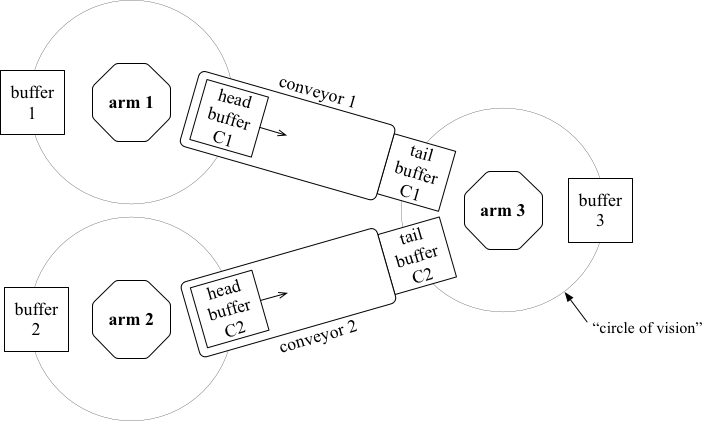
\includegraphics[width=0.7\textwidth]{imgs/scenario.png}
\caption[Scenario overview]{Schematic overview of the environment used. The figure depicts the entities involved and their relationship. The circle around the arms is referred as "the circle of vision".}
\label{fig:scenario}
\end{figure}

During the simulation and at each time step, the agents controlling the arms must select one action from their respective action space. At minimum, they all have access to the state information relative to the entities in their "circle of vision" as well as their own internal state to make their decision. The circle of vision is depicted in figure~\ref{fig:scenario} by the circle around each arm. $agent_{arm1}$ has guaranteed access to the state of $B_1$, $HBC_1$ as well as the position of the conveyor 1. Indeed, the position of the conveyor is required to know the availability status of the head buffer. The observation space of $agent_{arm2}$ is similar. $agent_{arm3}$'s observation space contains the state of $TBC_1$ and $TBC_2$ as well as the state of $B_3$. 

It is assumed that all agents have access to a \textit{noop} action indicating that the agent does not wish to execute anything.   When communication is enabled, $agent_{arm3}$ is the only agent that need to take both physical actions and communication actions. Its physical action space is composed of (1) move cube from $TBC_1$ to $B_3$, (2) move cube from $TBC_2$ to $B_3$ and (3) $noop$. The action space of the feeding $arm_i$ for $i \in {1,2}$ is composed of (1) move cube from $B_i$ to $HBC_i$ and (2) $noop$.

$arm_3$ (\textit{receiving} arm) is slower compared to the \textit{feeding} arm $arm_1$ and $arm_2$. It takes the receiving arm 3 time steps to move a cube from a point to another while for the two feeding arm, a single time step is needed. This speed disparity removes possible intrinsic coordination between the feeding and receiving arms. 

The environment will move from $t$ to $t+1$ only after all actions selected at time $t$ have been applied to the environment. The execution of a selected action might be refused. This happens if the underlying physical arm is still executing a past action. For example, at $t_0$, the agent responsible for $arm_3$ decides to take action $a$ (corresponding to moving a cube from $p_1$ to $d_1$). Because the speed of transport for $arm_3$ is $3$, the underlying arm will not be responsive to any new action during $t_1, t_2$ and $t_3$. This means that the only action the agent should select during those time steps is the $noop$ action.

\section{Communication schemes}
\label{sec:communication-schemes}

Communication can be approached from two different stand points. At each time step, beside a physical action, a communicating agent will also select a communication symbol (or message) $v \subset V \in \mathbb{R} ^{K \times 1}$. The symbols are discrete elements taken from a vocabulary $V$ of size $K$. The selected message $v$ will then be transmitted to the other agents. It is assumed that the messages in the vocabulary are distinct. Then, based on both their individual observation and the messages received, the agents will be able to select a physical action. The used communication schema influences the time between the sending of a message and its reception by the other agents. The first approach inspired by \cite{mordatch_emergence_2017} uses an instantaneous channel. A message selected at time step $t$ is directly available to the other agents. On the other hand, communication can be delayed as described by \cite{foerster_learning_2016}. With this approach, a message selected at time step $t$ will only be available to the other agent at minimum at time step $t+1$. It is important to stretch that no prior signification is assigned to the vocabulary symbols. Meaning will be assigned during training time by the agents themselves. Figure~\ref{fig:com-channels} illustrates the differences between the two communication approaches. 

\begin{figure}[ht]
\centering
  \begin{minipage}[t]{0.5\textwidth} %trying to force figs apart
    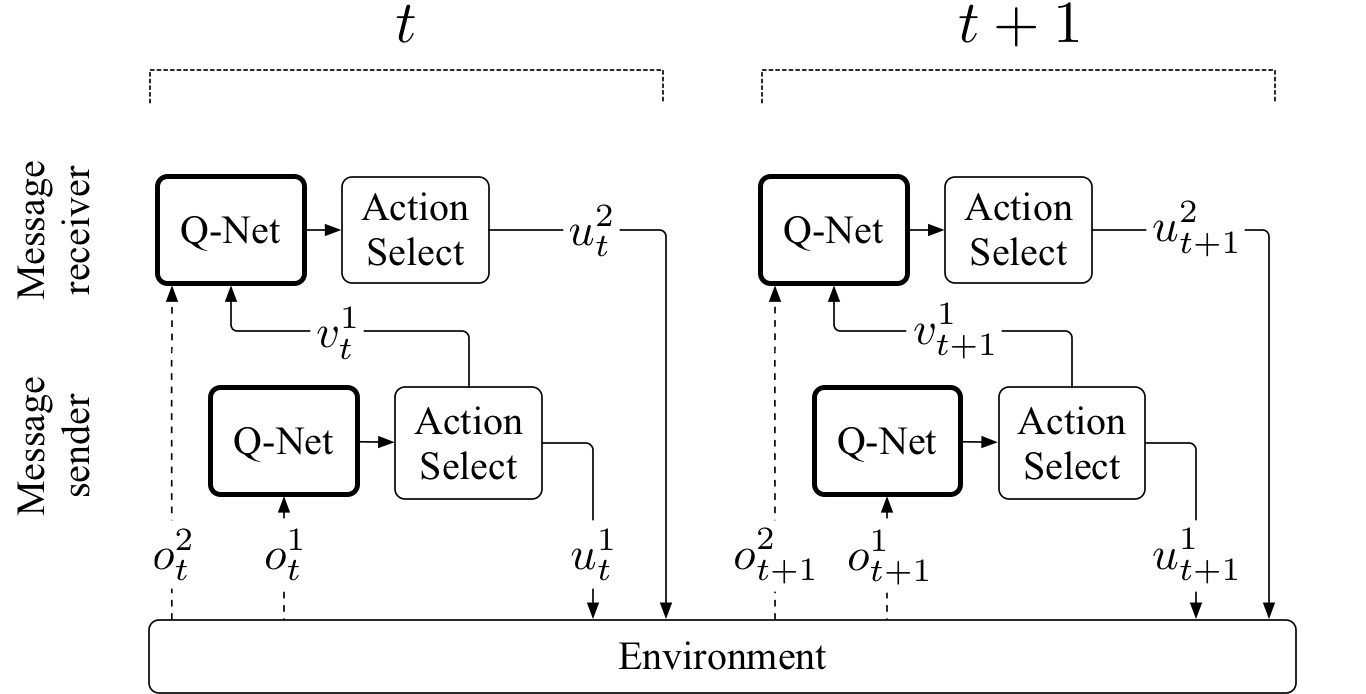
\includegraphics[width=\linewidth]{imgs/com-instant.png}
   % \caption*[Instantaneous communication scheme]{\textbf{Instantaneous communication} The message sent by a communicating agent are directly available to the other agents for their physical action selection.}
   \caption*{\textbf{Instantaneous communication} The message sent by a communicating agent are directly available to the other agents for their physical action selection.}
  \end{minipage}%
  \hfill
  \begin{minipage}[t]{0.5\textwidth}
    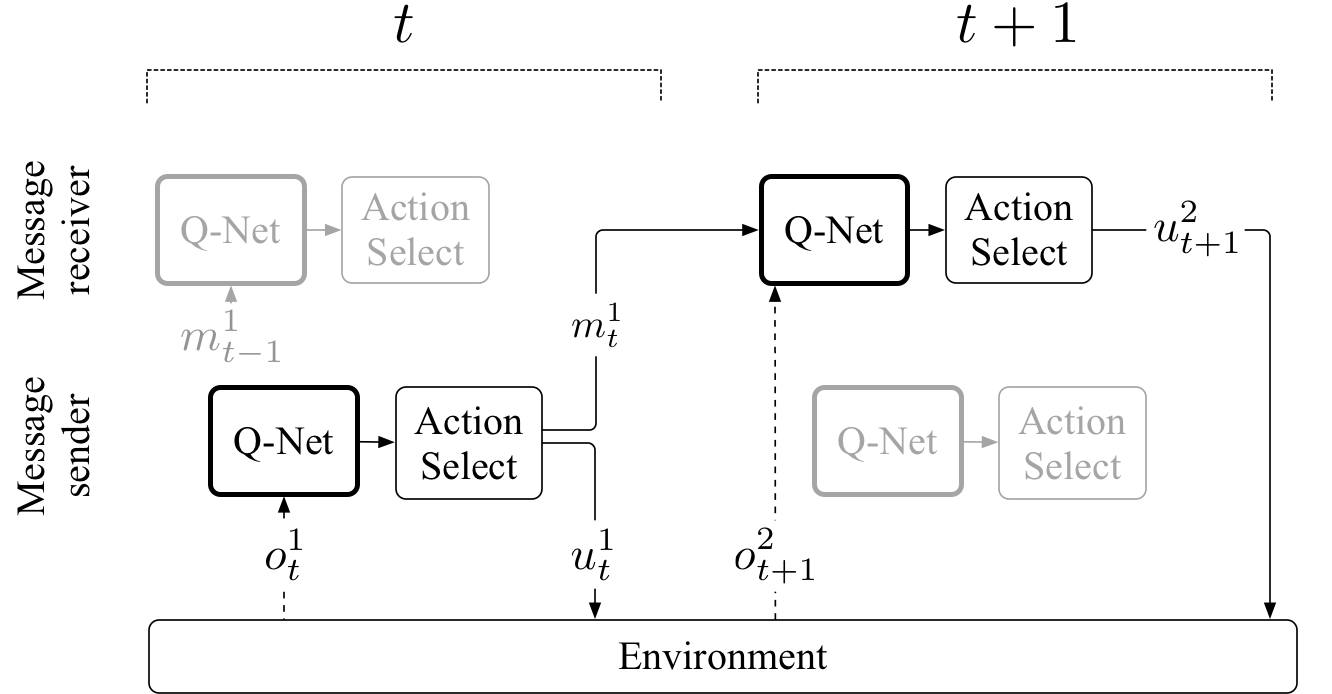
\includegraphics[width=\linewidth]{imgs/com-delay.png}
    %\caption*[Delayed communication scheme]{\textbf{Delayed communication} The message sent are available to the other agent at the following time step}
    \caption*{\textbf{Delayed communication} The message sent are available to the other agent at the following time step}
  \end{minipage}
  \caption{Comparison of process flow between instantaneous and delayed communication \protect\footnotemark}
  \label{fig:com-channels}
\end{figure}

\footnotetext{Figures are inspired by \cite{foerster_learning_2016}.}

In the experiments discussed in chapter~\ref{chap:discussion}, only $agent_{arm3}$ can communicate in a broadcast fashion to $agent_{arm1}$ and $agent_{arm2}$. Following the work of \cite{foerster_learning_2016}, $agent_{arm3}$ is separated into two sub-agents. One agent is used to select the communication action ($agent_{arm3c}$) and the other one to select the physical action ($agent_{arm3u}$). Both sub-agents share the same observation space. 

\section{Reward function}
\label{sec:reward-function}

The most straight forward reward would be related to the solving of the task. Unfortunately, initial experiments showed that this approach does not provide enough feedback to the agents to learn effectively. Instead, reward shaping is used. In order for the learner to strive for cooperative behaviour the reward signal is shared between the agents. The global reward is as follows:

\begin{equation}
    r_{t} = \sum_{a \in A_t} R(s_{t-1}, a, s_t) + r_{time}
\end{equation}

The global reward is hand-crafted from three sub-parts. As an incentive to avoid drop of cubes, a \textbf{cube reward} is added per cube transported during the time-step. A reward of $-1$ is given if the cube is dropped, $1$ otherwise. A selected action might give rise to a \textbf{behaviour reward} of $-1$ if it was not realised by the underlying arm. This signal is used to avoid flooding of the meta controller by the learners with actions that can not be fulfilled. For example, this situation can happen when the underlying arm is still moving. An additional fixed reward ($r_{time}$) is added to he global reward for every elapsed time-step. A negative \textbf{time reward} can be used to push agents to be active and finish the task as soon as possible.

\begin{equation*}
    R(s_{t-1}, a, s_t) = c(s_{t-1}, a, s_t) + b(s_{t-1}, a, s_t)\\
\end{equation*}

\begin{equation*}
\begin{array}{rl}
    c(s_{t-1}, a, s_t) = & \left\{
     \begin{array}{rl}
       -1 & : \text{action $a$ resulted in a drop of cube}\\
       +1 & : \text{action $a$ resulted in a correctly transported cube} \\
       0 & :  \text{otherwise}
     \end{array}
    \right. \\
    b(s_{t-1}, a, s_t) = & \left\{
     \begin{array}{rl}
       -1 & : \text{action $a$ was not executed (refused)}\\
       0 & :  \text{otherwise}\\
     \end{array}
   \right.
\end{array}
\end{equation*}

On top of the shared reward, a individual \textbf{communication reward} ($r_{com}$) can be added. The communication reward is related to usage cost of the channel. It might be positive to favour usage of the channel or negative to favour communication scarcity. It is assumed that the vocabulary at the disposal of a communicating agent contains an equivalent to "no message sent" which incurs no cost. This enables the learner to decide if sending a message is worth the cost.

\section{Training}

One training session is composed of 6000 episodes. An episode corresponds to one transport session happening in the environment described above. Before each episode, the world is reset. All cubes still present are removed and all robotic arms are reset. Afterwards, each buffer is filled with a random number of cubes. The number of cube put into each buffer follows a normal distribution $\mathcal{N}(\mu=0.75*\textit{max buffer size}, \sigma=3)$. An episode is considered finished either when a predetermined number of time steps has been done or when no cube are left to transport  (all cube have either reached buffer 3 or have been dropped). Chapter~\ref{chap:discussion} presents a comparison between learning scenarios as well as the influence of the different hyper parameters on the learned solutions. In order to evaluate the efficacy of the policies learned, the resulting learners are applied to $500$ new random problems. The learning process is repeated $50$ times. A solution is considered optimal if during the 500 evaluation problems 100\% of the cube to be transported reach buffer 3 ($B_3$).

\subsection*{Centralised Learning}

This approach uses a single agent making decisions based on a concatenation of all observation and action space of all agents. With this approach there is no autonomy of agents and the multi-agent task is transformed in a single agent task. The centralised learning is used as one of the baselines.

\subsection*{Decentralised Learning}

When decentralised learning is used, each arm is managed by an autonomous agent learning at the same time in the same task. Both decentralised learning with full and partial observability are explored. In order to circumvent the inability of the agents to have a direct insight about the other agent behaviours in the partial observability case, communication is used.

\subsection{Action selection and exploration}

Learners are all implemented using vanilla tabular Q-learning with optimistic initialisation. The discount factor used during learning will be indicated for each experiment. The actions are selected to be the maximum estimated Q-Value relative to a given observation, $a = \argmax_a q(o, a)$. In order to maintain exploration during training, an $\epsilon$-greedy policy is used with an exploration rate decreasing linearly over time from 0.5 to 0.05.













% # Instantaneous communication analysis

% ## Perfect channel
% Table Optimality (rwdt, disc + costless com)
% Optimality per variable (rwdt, disc + costless com)

% Table com-compelexity (rwdt, disc + costless com)
% Com-complexity per variable (rwdt, disc + costless com)

% Grounding of communication:
% - Look only at optimal resolutions

% Usage of zero by AC based on communication cost state [1,1], [1,0], [0,1] (can receive) make into relation with number of optimal
% Reaction to message i.e. meaning of received message


% # SIMULATION TO DO
% ## Unperfect channel (drop)
% - Drop rate (best disc, best com-r, best time-r)
% - Com-msg (2,3,4,8)


% -  MARLAO Busoniu p21 for justification for Q-Learning



 % Experimental Setup
\chapter{Results \& Discussion}
\lhead{\emph{Results \& Discussion}} 
\label{chap:discussion}

In order to add stochasticity to the learning, $arm3$ is controlled by a scripted agent. When $agent_{arm3}$ has the ability to transport a cube, it will do so with 50\% chance. 

%This approach strengthens the assumption that the different agents can not find an hidden synchronisation mechanism beside the communication.

\section{Learning approach comparison} 

Table~\ref{tab:exp-0-comparison} demonstrates the veracity of the assumption made in the introduction. The best hyperparameters are used for the training. The best hyperparameters are selected by looking at which parameters maximise $\frac{\textit{ratio of sinked cube}}{\textit{ratio of dropped cube}}$. The simulated problem can be solved optimally when the agents have full observability in a reliable manner. The learning can then be done in a centralised ($CFO$) or decentralised ($DFO$) manner. Removing the agent's access to the full observability of the environment makes the problem unsolvable ($DLO$). Figure~\ref{fig:exp-0-comparision} also shows that with $DLO$ learning, the agents have a tendency to transport cubes even though they do not have certainty about the outcome of their action. This behaviour is studied in-depth in section~\ref{sec:risk-aversion}. Also, table~\ref{tab:exp-0-comparison} confirms that introducing instantaneous communication can help mitigate the partial observability problem ($DLOCI$) and help solving optimally the problem.


\begin{table}[ht]
\centering
\begin{tabular}{lrr}
\toprule
Training method  &            &  Optimality      \\
\midrule
Centralised & $CFO$  & 1.00 \\
Dec. Full obs. &  $DFO$  & 1.00 \\
Dec. Limited obs. & $DLO$  & 0.00 \\
Dec. Limited obs. with delayed com. ($\abs{V}  = 2$) & $DLOCD$ & 0.00 \\
Dec. Limited obs. with instantaneous com. ($\abs{V}  = 2$) & $DLOCI$ & 0.82 \\
\bottomrule
\end{tabular}
\caption[Optimality ratio relative to the training method]{Optimality ratio relative to the training method}
\label{tab:exp-0-comparison}
\end{table}


\begin{tabular}{lr}
\toprule
Method         &  Optimality      \\
\midrule
$CFO$  & 1.00 \\
$DFO$  & 1.00 \\
$DLO$  & 0.00 \\
$DLOCI$ & 0.82 \\
\bottomrule
\end{tabular}


\begin{tabular}{lrr}
\toprule
$TBC1$ state & $TBC2$ state & Intent enc.\\
\midrule
Emtpy & Empty & (11)  \\
Emtpy & Full &  (10) \\
Full & Emtpy & (01) \\
Full & Full & (00) \\
\bottomrule
\end{tabular}



\begin{figure}[ht]
\centering
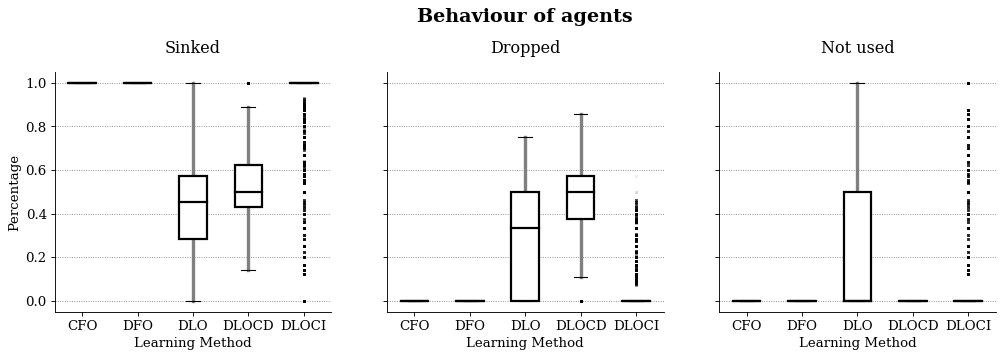
\includegraphics[width=\textwidth]{imgs/exp-0-comparision-fo-lo.png}
\caption[Behaviour of agents relative to training method]{Behaviour of the agents relative to the training method. For each method, the best hyper parameters are used\protect\footnotemark.}
\label{fig:exp-0-comparision}
\end{figure}

\footnotetext{Figure \ref{fig:exp-0-comparision} is constructed from $50$ training session each composed of $500$ evaluation problems. The reparation of cube usage observed in each problem is then aggregated and transcribed in the figure. Hyper parameters used: $CFO$ ($\gamma=0.9$, $r_{time}=-0.1$), $DFO$ ($\gamma=0.9$, $r_{time}=-0.1$), $DLO$ ($\gamma=0.9$, $r_{time}=0.0$, $r_{com}=0.0$), $DLOCD$ ($\gamma=0.9$, $r_{time}=-0.1$, $r_{com}=-0.1$), $DLOCI$ ($\gamma=0.9$, $r_{time}=0.0$, $r_{com}=0.0$).}

Interestingly, in the simulated problems, having a delayed communication ($DLOCD$) precludes the learning of optimal solutions. This might be explained by the absence of a direct link between communication and resulting action. With a delayed communication, a received reward at time $t$ might be related to a communication made at time $t-1$. As a result, it is more difficult for the agents to agree on a grounding of the communication. \cite{foerster_learning_2016} relies on centralised learning and decentralised execution to mitigate this problem. This approach to MARL being out of the scope of this work, instantaneous communication is used in the following analysis.

In order for the agent to have an incentive to transport cubes and to take into account their past action, a time-reward of $-0.1$ and a discount factor of $0.9$ will be used as default values in the subsequent parts of the discussion. 

\section{Risk aversion}
\label{sec:risk-aversion}
When communication is not available and control is decentralised, agents must take action with a much higher degree of uncertainty. The uncertainty raises from the absence of state information about the tail buffer of the conveyors for $agent_{arm1}$ and $agent_{arm2}$.  In the $DLO$ scenario, no optimal solutions are found and a certain number of solutions results in drop of cubes. As reflected in figure~\ref{fig:exp-0-comparision}, they still have a tendency to transport cubes without the guarantee of a positive outcome. 

In a specific training session, an agent is considered to be \textit{risk averse} if it does not perform any other action than $noop$ and \textit{risk seeking} otherwise. The risk aversion of an agent can be seen as a measure of the trade -off between selecting an action with an unknown payoff compared to another one with a possibly lower, but more predictable payoff. 

The $DLO$ setting is particularly suited to study the risk aversion of the agents. Indeed, in this setting both $agent_{arm1}$ and $agent_{arm2}$ have no opportunity to coordinate with respect to the state of the tail buffer of the conveyors. Figures~\ref{fig:exp-1-risk-rwdt} and \ref{fig:exp-1-risk-disc} show the average risk aversion. The risk aversion is calculated by looking at the learned behaviour of both $agent_{arm1}$ and $agent_{arm2}$. The risk aversion represents the ratio of solutions where both agents are risk averse, i.e do not transport any cubes. A risk aversion of $1$ means that in 100\% of the training sessions, both  $agent_{arm1}$ and $agent_{arm2}$ learned to not transport cubes. On the other hand, a risk aversion of $0$ indicates that in all the training sessions both agents were risk seeking and learned to send cube under uncertainty.

\begin{figure}[H]
\centering
\begin{minipage}[t]{.5\textwidth}
  \centering
  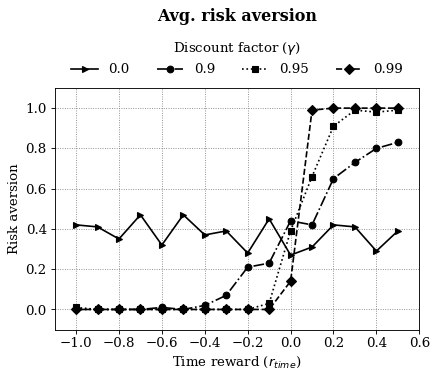
\includegraphics[width=\linewidth]{imgs/exp-1-risk-rwdt.png}
  \caption[Average risk aversion relative to the time-reward]{Average risk aversion relative to the time-reward.}
  \label{fig:exp-1-risk-rwdt}
\end{minipage}%
\begin{minipage}[t]{.5\textwidth}
  \centering
  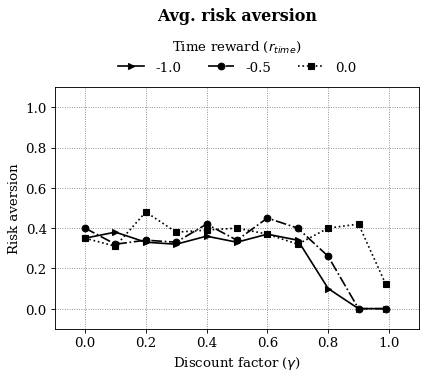
\includegraphics[width=\linewidth]{imgs/exp-1-risk-disc.png}
  \caption[Average risk aversion relative to the discount factor]{Average risk aversion relative to the discount factor.}
  \label{fig:exp-1-risk-disc} 
\end{minipage}
\end{figure}

Acting as a sanity check, when both the time reward and the discount factor are bigger than $0$ the agents have a high risk aversion. The positive time reward pushes the arm to "run the clock". By not transporting any cube, they wait until the maximum number of time steps is reached and as a result maximise the long term return. On the other hand, as long as the agent's horizon is not too long, the time reward does not seem to influence the risk aversion (fig.~\ref{fig:exp-1-risk-disc}). At the extreme, the discount factor of $0$  the time reward only shifts all Q estimates by the same amount. As the discount factor gets closer to 1, the arms become more risk seeking. With the goal of maximising the long term reward, any transported cube will make the episode finish faster. In addition to shortening the episode, a few cubes might be transported correctly which increases the total long term reward. 

%%%%%%%%%%%%%%%%%%%%%%%%%%%%%%%%%%%%%%%%%%%%%%%%%%%%%%
%%%%%%%%%%%%%%%%%%%%%%%%%%%%%%%%%%%%%%%%%%%%%%%%%%%%%%
%%%%%%%%%%%%%%%%%%%%%%%%%%%%%%%%%%%%%%%%%%%%%%%%%%%%%%
%%%%%%%%%%%%%%%%%%%%%%%%%%%%%%%%%%%%%%%%%%%%%%%%%%%%%%

\section{Communication Analysis}

\subsection{Influence of communication reward}

The cost related to the channel usage is introduced by adding a communication reward to the global reward for $agent_{arm3c}$. As explained in section \ref{sec:reward-function}, the communication reward is only added to the sender. As a reminder, the messages in the vocabulary from which the communication agent picks are labelled from $0$ to $\abs{V} - 1$. The usage of the message $v_0$ incurs no cost as it is the equivalent to "no message sent". In order to facilitate the analysis of the influence of the communication reward in the $DLOCI$, a vocabulary of size $2$ is used. 

\begin{figure}[H]
\centering
\begin{minipage}[t]{.5\textwidth}
    \centering
    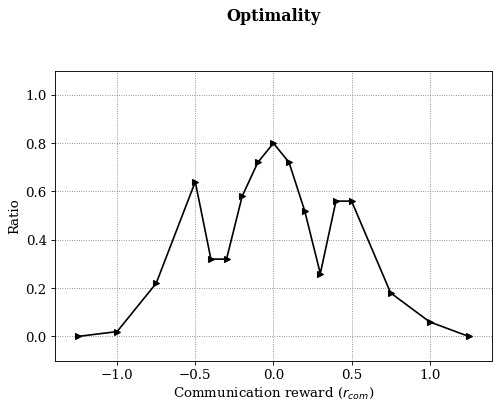
\includegraphics[width=0.95\textwidth]{imgs/exp-2-rwdc-2msg-optimality.png}
    \caption[Influence of $r_{com}$ on optimality of learning]{Optimality of learning when trained with hyperparameters $\abs{V}=2$, $r_{time}=-0.1$ and $\gamma=0.9$ relative to the cost of communication.}
    \label{fig:exp-2-rwdc-optimal}
\end{minipage}%
\begin{minipage}[t]{.50\textwidth}
    \centering
    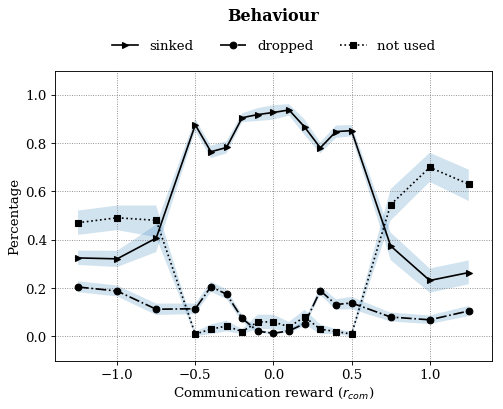
\includegraphics[width=0.95\textwidth]{imgs/exp-2-rwdc-2msg-behaviour.png}
    \caption[Influence of $r_{com}$ on the behaviour of the agents]{Behaviour of the agents when trained with hyperparameters $\abs{V}=2$, $r_{time}=-0.1$ and $\gamma=0.9$ relative to the cost of communication.}
    \label{fig:exp-2-rwdc-behaviour}
\end{minipage}
\end{figure}

Figures~\ref{fig:exp-2-rwdc-optimal} and \ref{fig:exp-2-rwdc-behaviour} shows that the ratio of optimal solution drops to 0 when the absolute value of the communication reward is too high. With such a communication reward, the agents reach a sub-optimal Nash equilibrium. $Agent_{arm3c}$ will learn to always send a specific message from the vocabulary depending on the sign of the communication reward. It will do so in order to maximise its own reward. Following convergence, an improvement in the solution can only be expected if all agents change their behaviour. One can see that with only two messages available the most reliable learning is done with a cost-less or an almost cost-less communication channel (i.e. $r_{com}\approx0$). With no implicit constraint on the usage of the vocabulary there is a higher chance than the agents will converge to a optimal solution. The behaviour is similar for $\abs{v}=4$ when $t_{com} \leq 0$. When $t_{com} > 0$, the drop in optimality is not seen. Indeed, $agent_{arm3c}$ can now discard the use of $v_0$ and still have access to a sufficient vocabulary size to solve the problem optimally.

%\todo{Dip of the optimality around +- 0.25 => why?}

\subsubsection*{Grounding of communication}

Grounding of communication between interacting entities is a widely researched topic. First introduced by Clark, Herbert H. and Brennan, Susan E. (1991) \cite{resnick_grounding_1991}, it relates to the collection of "mutual knowledge, mutual beliefs, and mutual assumptions" that is required for successful communication between two entities. A common grounding criterion is that everyone involved has a clear enough understanding of the concept and intent transported through the communication channel to move forward correctly \cite{horvitz_grounding_2000}. Also, in the setting of reinforcement learning, a link with the \textit{new contribution} method proposed by \cite{clark_contributing_nodate} to reach grounding of communication can be made. This method relies on a partner moving forward with a new idea and waiting to see if its partners expresses confusion. In reinforcement learning, this can be seen as sending a specific message and looking at the resulting reward. The reward then acts as an indication of the confusion of the other agents \cite{koschmann_reconsidering_2003}.

\begin{table}[H]
    \centering
    \begin{tabular}{lrrr}
        \toprule
        $TBC1$ state & $TBC2$ state & Intent enc. & Who can transport safely a cube? \\
        \midrule
        Emtpy & Empty & (11) & Both feeding arms \\
        Emtpy & Full &  (10) & Only $arm1$ \\
        Full & Emtpy & (01) & Only $arm2$ \\
        Full & Full & (00) & Not safe for both \\
        \bottomrule
    \end{tabular}
    \caption[Abstracted sub states for $agent_{arm3c}$]{Abstracted sub states for $agent_{arm3c}$. The sub states represents the possible intents that can be transmitted though the communucation channel.}
    \label{tab:agent3c-substate}
\end{table}

The grounding of communication focuses on the interconnection between the intent of the message sent and its interpretation by the receiving agents. Only protocols resulting in optimal solution will be studied. The protocols are inferred from the learned Q-Table. An optimal solution guarantees that at least one message is sent with the intent to indicate that it is not safe for both agents to transport a cube and interpreted correctly. It is important to note that even tough the intent of a message might be "safe for both", in reality $agent_{arm1}$ interprets this message as "safe for me" as it has no notion of existence of $agent_{arm2}$. The same can be said for the interpretation at $agent_{arm2}$. It is only when looking at the intent of the message and the reaction of both feeding arm to the message that it is possible to determine the overall grounding of the protocol.

The state space of $agent_{arm3c}$ is not limited to the status of the buffer $TBC1$ and $TBC2$. Consequently, the communicating agent could send more than a one symbol per sub state. However, it will have to do it at different time steps. The sub state can be seen as a categorisation on top of the state of $agent_{arm3c}$. For example, $agent_{arm3c}$ can be in sub state $00$ while the underlying arm is moving or not which gives two different states. Also, $agent_{arm3c}$ can send the same message $v$ in different sub states.

The grounding of the communication can be represented by a tripartite graph. Figure~\ref{fig:protocol-2msg-good} depicts an example of such a graph. The nodes on the left side represent the intent of the message sent which is related to the sub states shown in table~\ref{tab:agent3c-substate}. The nodes on the right correspond to the interpretation of the message by $agent_{arm1}$ and $agent_{arm2}$. Both the intent and the interpretation are encoded using a binary representation. A "$1$" indicates "safe to transport" and a "$0$" indicates "not safe to transport". For example, "$10$" on the intent side means that it is safe for $agent_{arm1}$ to transport a cube while it is not for $agent_{arm2}$. On the other hand, "$10$" on the interpretation side means that $agent_{arm1}$ interprets the message as "safe for me to transport" while  $agent_{arm2}$ interprets it as "not safe for me to transport". Finally, the nodes in the middle represent the vocabulary. The example presents a possible grounding of communication leading to an optimal solution when $\abs{V} = 2$. This type of protocol only transmits two intents through the channel: the fact that both feeding arms can send safely as well as the opposite. Each intent correctly transmitted though the channel is represented by a coloured node on both side of the graph. A dashed arrow depicts an intent not correctly interpreted by at least one of the the feeding agents. When the number of intent correctly transmitted is equal to the number of available symbols, the protocol will be called ideal, otherwise non-ideal. 

\begin{figure}[H]
\centering
\begin{minipage}[t]{.5\textwidth}
  \centering
  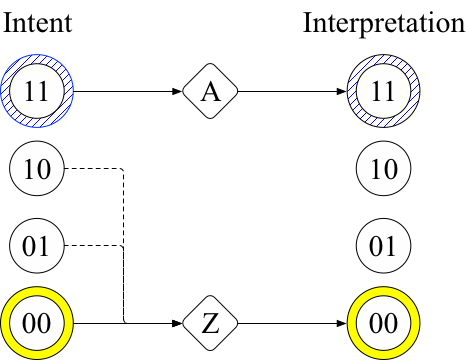
\includegraphics[width=.85\linewidth]{imgs/protocol-2msg-good.png}
  \caption[Ideal protocol for $\abs{V} = 2$]{Example of an ideal protocol for $\abs{V} = 2$ leading to an optimal solution.}
  \label{fig:protocol-2msg-good}
\end{minipage}%
\begin{minipage}[t]{.5\textwidth}
  \centering
  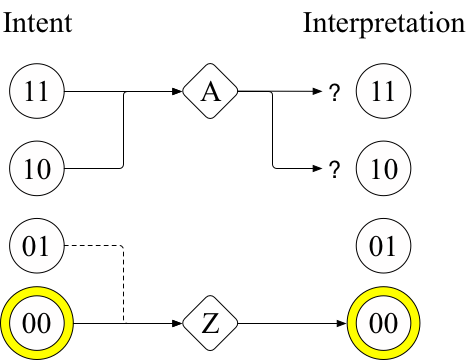
\includegraphics[width=.85\linewidth]{imgs/protocol-2msg-bad.png}
  \caption[Misinterpreted protocol for $\abs{V} = 2$]{Example of protocol for $\abs{V} = 2$ leading to a sub-optimal solution.}
  \label{fig:protocol-2msg-bad}
\end{minipage}
\end{figure}

Out of the 16 possible types of protocol, only five types can lead to an optimal solution (see fig.~\ref{tab:exp-2-assigments-distrib} for the list). In order to distinguish them, a binary encoding of the intents correctly interpreted is used. Each digit of the binary strings of length $4$ represents one of the intent present in table~\ref{tab:agent3c-substate}. If the related intent is correctly transmitted and interpreted, a $1$ will be present in the encoding, otherwise $0$ is used. The example above thus result in the encoding $1001$. We distinguish between the protocol type and the protocol itself. A protocol type indicates which intent is correctly interpreted. On the other hand, a protocol is a realisation of a protocol type where the symbols of the vocabulary have been assigned to a specific vocabulary node in the graph.

It is clear that with a vocabulary of size $2$ the only grounding leading to an optimal solution is based on the protocol type $1001$.  As a result, there exists only two valid protocols and both are ideal protocols. A valid protocol is a protocol leading to an optimal solution. They correspond to the two different assignments of the symbols of the vocabulary to the node $A$ and $Z$. One where the symbol $v_1$ is assigned to node $A$ and $v_0$ to node $Z$ and the opposite. Figure~\ref{fig:protocol-2msg-bad} depicts an invalid protocol. Compared to before, $agent_{arm3c}$ also tries to convey information about the sub sate "safe for $arm1$ but not safe for $arm2$" via symbol $A$. Because of this change in the protocol, it is now impossible for $agent_{arm2}$ to decipher whether it is safe to transport a cube or not. For $agent_{arm2}$, symbol $A$ now indicates that $TBC2$ can either be full or empty. As a result $agent_{arm2}$ can no longer definitively know the intent conveyed by $A$. In this situation, $agent_{arm2}$ can not know the state of $TBC2$ with certainty. As a result will either learn to not send any cube or send cube by becoming risk seeking. Either way, this will result into a non optimal solution with less than 100\% of the cube sinked.

\subsubsection*{Influence of communication-reward on the grounding of communication}

When looking at optimal solutions with a vocabulary of size $2$ $V = (v_0, v_1)$ over a perfect channel,  the communication reward influences the meaning that the agents agree to attribute to specific symbols (fig.~\ref{fig:exp-2-rwdc}). When the cost of using the channel is greater than $0$, the communicating agent has an incentive to use the costly message ($v_1$) when there are no possibilities of receiving any other positive reward. As a result, $v_1$ will be used to indicate the intent "$00$" (i.e. "not safe to transport for both"). On the other hand, when the cost is lower than $0$, the inverse happens. The agents will converge to a grounding of the communication using the costly message ($v_1$) to indicate that both feeding arms can transport cube safely. The positive reward received after a successful transport is used to compensate the usage cost of the channel. When there is no cost in using either word of the vocabulary, no preference in the grounding of the protocol is seen. Half the time the costly symbol will convey information that will push the feeding agents to transport and the other half will indicate they should not move.

\begin{figure}[H]
\centering
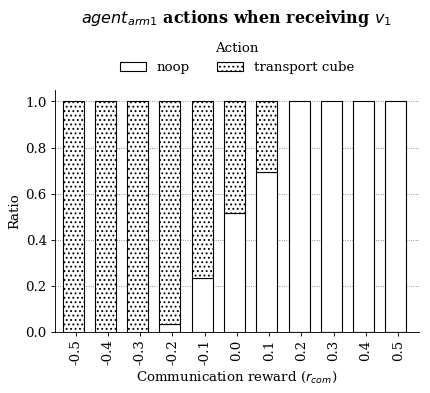
\includegraphics[width=0.5\textwidth]{imgs/exp-2-rwdc-2msg-grounding-a1.png}
\caption[Grounding of communication relative to $r_{com}$ for \abs{v}=2]{$agent_{arm1}$ reaction to receiving message $v_1$. Only looks at state where $agent_{arm1}$ could potentially transport a cube.}
\label{fig:exp-2-rwdc}
\end{figure}

%%%%%%%%%%%%%%%%%%%%%%%%%%%%%%%%%%%%%%%%%%%%%%%%%%%%%%
%%%%%%%%%%%%%%%%%%%%%%%%%%%%%%%%%%%%%%%%%%%%%%%%%%%%%%
%%%%%%%%%%%%%%%%%%%%%%%%%%%%%%%%%%%%%%%%%%%%%%%%%%%%%%
%%%%%%%%%%%%%%%%%%%%%%%%%%%%%%%%%%%%%%%%%%%%%%%%%%%%%%

\subsection{Vocabulary size}

Until now, only solutions with the minimum amount of symbols necessary to solve the task were considered. As shown before, not all possible protocol graphs and assignments of the vocabulary can lead to an optimal solution and considered valid. The number of valid protocols relative to the size of the vocabulary is shown in table~\ref{tab:exp-2-assigments}. 

\begin{table}[H]
\centering
\begin{minipage}[t]{.5\textwidth}
    \centering
    \begin{tabular}{lrr}
    \toprule
    $\abs{V} $ & \multicolumn{2}{c}{Valid assignments} \\
    \midrule
    $2$ & 12.5\% & (2/16)\\
    $3$ & 37.5\% & (24/64)\\
    $4$ & 57.8\% & (146/256)\\
    $8$ & 89.2\% & (58466/65536)\\
    \bottomrule
    \end{tabular}
    \caption[Number of valid vocabulary assignments]{Number of valid vocabulary assignments relative to the size of the vocabulary. Representation: (valid protocols/ possible protocols)}.
    \label{tab:exp-2-assigments}
\end{minipage}%
\begin{minipage}[t]{.50\textwidth}
    \centering
    \begin{tabular}{lr}
    \toprule
    $\abs{V} $ &  optimality \\
    \midrule
    2.0 &   0.78 \\
    3.0 &   1.00 \\
    4.0 &   0.94 \\
    8.0 &   0.96 \\
    \bottomrule
    \end{tabular}
    \caption[Optimality ratios with default hyperparameters relative to vocabulary size]{Optimality ratio for 50 training session with hyperparameters $r_{time}=-0.1$, $r_{com}=-0.1$ and $\gamma=0.9$}
    \label{tab:exp-2-vocabulary-optimal}
\end{minipage}
\end{table}

As shown in table~\ref{tab:exp-2-vocabulary-optimal}, the increase in vocabulary size also brings an increase in the probability of getting an optimal solution at the end of a training session. With a bigger vocabulary there is a higher chance to converge to an optimal solution compared to $\abs{V}=2$. For $\abs{V}=2$, a single misinterpretation will make the solution sub-optimal. 

When more than two words are available, most valid protocols can be simplified. Even tough the agents could convey more than two intents through the channel, it is not required to solve the problem optimally. In case the sender is not precise enough or the receivers are not able to learn correctly the intent of each symbol, it might be possible to discard the intent or the symbol altogether.

\subsubsection*{Complexity}

As representation of the complexity of a learned protocol, the number of intents that are correctly interpreted is used. As a result, in order to achieve the maximum complexity the vocabulary needs to be composed of a minimum of 4 symbols. Table~\ref{tab:exp-2-assigments-distrib} shows the different types of protocol and their respective ratio out of the pool of valid protocols \footnote{The assignments are generated using random sampling of possible protocols. Each generated protocol is then checked to see if it can lead to an optimal solution. If it is the case, the type of protocol is then determined.}.


\begin{table}[H]
 \centering
    \begin{tabular}{lrrrr}
    \toprule
    Protocol type & $\abs{V}  = 2$ & $\abs{V}  = 3$ & $\abs{V}  = 4$ & $\abs{V}  = 8$ \\
    \midrule
    $0111$ & 0 & \underline{25\%} & 24.6\% & 9.9\% \\
    $1001$ & \underline{100\%}\ & 25\% & 9.5\% & 9.9\% \\
    $1011$ & 0 & \underline{25\%} & 24.6\% & 4.3\% \\
    $1101$ & 0 & \underline{25\%} & 24.6\% & 9.9\% \\
    $1111$ & 0 & 0 & \underline{16.4\%} &  \underline{69.8\%} \\
    \bottomrule
    \end{tabular}
    \caption[Distribution of protocol type]{Distribution of the type of protocols relative to the vocabulary size. For each vocabulary size, ratios relative to ideal protocols are underlined. }
    \label{tab:exp-2-assigments-distrib}
\end{table}

Figure~\ref{fig:exp-2-assigments} shows that even though the vocabulary size increases, it is not guaranteed that the learned protocol will be complex or ideal. Also, the agents do not ground the learned protocols uniformly. In most of the training sessions, the intent conveyed by the learned protocol is limited to $01$, $10$ and $11$ (protocol $0111$). 

\begin{figure}[H]
\centering
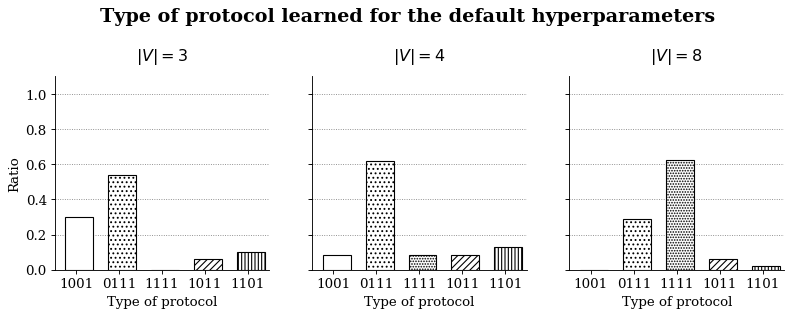
\includegraphics[width=\textwidth]{imgs/exp-2-complexity-default-comparison.png}
\caption[Empirical distribution of protocol types (default parameters)]{Empirical distribution of protocol types for 50 training sessions with hyperparameter $r_{time}=-0.1$, $r_{com}=-0.1$, $\gamma=0.9$}
\label{fig:exp-2-assigments}
\end{figure}

The protocols have thus a tendency to only convey individual safety intent except when the vocabulary size is greater than the number of possible intents. In this setting, the protocol is more often ideal (indicates all intents, i.e. protocol type $1111$). This behaviour can probably be attributed to the fact that the protocol $1111$ is the most common assignment for $\abs{V} = 8$.

An example of a learned protocol with a non-ideal usage of a vocabulary of size $4$ is depicted in \ref{fig:protocol-4msg-bad}. In this example $agent_{arm3c}$ tries to convey to two intents via symbol $A$. Contrary to $agent_{arm2}$, $agent_{arm1}$ can correctly interpret symbol $A$. For $agent_{arm1}$, the symbol $A$ always indicate that it is safe to transport a cube. On the other hand, symbol $A$ conveys two contradictory intents to $agent_{arm2}$ and as a result the agent will not be able to leverage the received communication for its decision process. An ideal protocol with 4 messages can be found in figure~\ref{fig:protocol-4msg-good}. With such protocol, all messages indicate a different sub state and the vocabulary is maximally used.

\begin{figure}[H]
\centering
\begin{minipage}[t]{.5\textwidth}
    \centering
    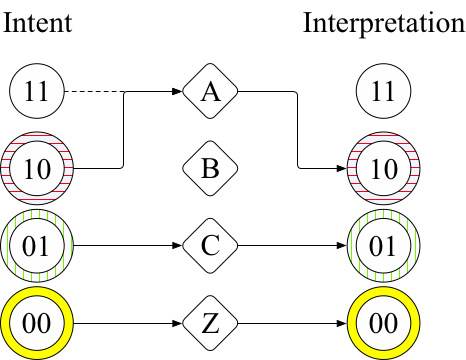
\includegraphics[width=0.95\textwidth]{imgs/protocol-4msg-low.png}
    \caption[Non-ideal communication protocol for $\abs{V} = 4$]{Non-ideal communication protocol for $\abs{V} = 4$ (protocol type : $0111$)}
    \label{fig:protocol-4msg-bad}
\end{minipage}%
\begin{minipage}[t]{.50\textwidth}
    \centering
    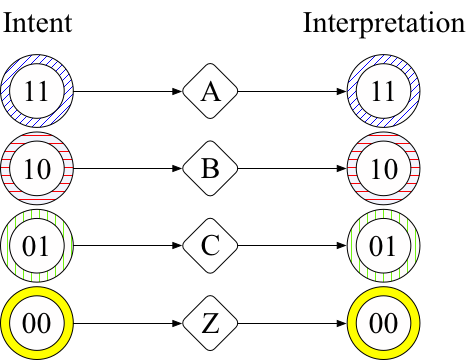
\includegraphics[width=0.95\textwidth]{imgs/protocol-4msg-high.png}
    \caption[Ideal communication protocol for $\abs{V} = 4$]{Ideal communication protocol for $\abs{V} = 4$ (protocol type : $1111$)}
    \label{fig:protocol-4msg-good}
\end{minipage}
\end{figure}

\subsubsection*{Influence of the discount factor on complexity}

The ratio of solutions with an ideal protocol (fig.~\ref{fig:exp-2-disc}) can be increased by lowering the discount factor. By being myopic, the goal is to receive a positive reward as often as possible. In our experiments, a positive reward is received each time a cube is transported correctly. As a result, a low discount rate pushes $agent_{arm3c}$ to indicate as soon as possible an empty buffer. Also, the grounding of communication is facilitated as the estimated Q function contains less noise coming from decisions made in different states. At the extreme, with a discount rate of 0, the agents receive a direct feedback about the quality of the communication. This increase is visible for all vocabulary size as shown in figure~\ref{fig:exp-2-disc-best}.

%\todo{justify parameter selection for gamma}

\begin{figure}[ht]
\centering
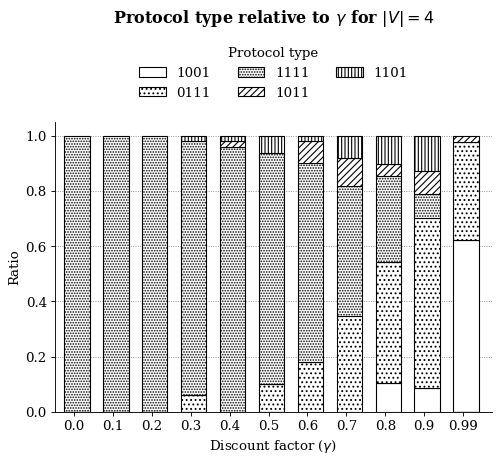
\includegraphics[width=0.6\textwidth]{imgs/exp-2-complexity-4msgs-discount.png}
\caption[Empirical distribution of protocol types relative to the discount rate]{Distribution of protocol types relative to the discount rate for $\abs{v}=4$.}
\label{fig:exp-2-disc}
\end{figure}

\begin{figure}[ht]
\centering
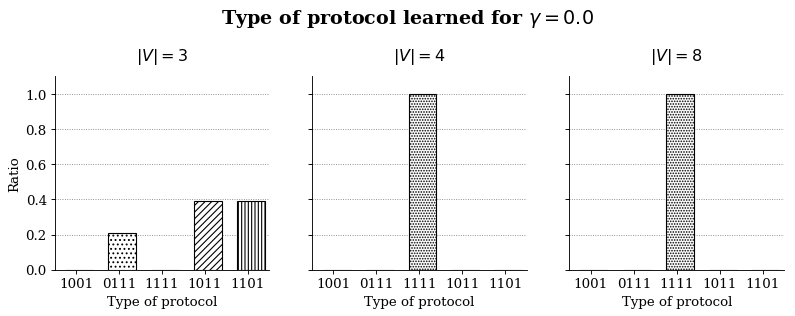
\includegraphics[width=\textwidth]{imgs/exp-2-complexity-best-comparison.png}
\caption[Empirical distribution of protocol types (best parameters)]{Empirical distribution of the protocol type for 50 training sessions with hyperparameter $r_{time}=-0.1$, $r_{com}=-0.1$, $\gamma=0.0$}
\label{fig:exp-2-disc-best}
\end{figure}

% %%%%%%%%%%%%%%%%%%%%%%%%%%%%%%%%%%%%%%%%%%%%%%%%%%%%%%
% %%%%%%%%%%%%%%%%%%%%%%%%%%%%%%%%%%%%%%%%%%%%%%%%%%%%%%
% %%%%%%%%%%%%%%%%%%%%%%%%%%%%%%%%%%%%%%%%%%%%%%%%%%%%%%
% %%%%%%%%%%%%%%%%%%%%%%%%%%%%%%%%%%%%%%%%%%%%%%%%%%%%%%

\section{Unreliable channel}

Up to now, the channel has been assumed to be fully reliable. As a result not sending a message can be seen as a standalone word of the vocabulary. Moving to an unreliable channel which can drop messages introduces a prerogative on the usage of the channel. The message $v_0$ ("no message sent") must now be grounded as intent "$00$" (i.e "not safe for both"). Indeed, if any of the feeding agent ground the communication differently, a dropped message might be misinterpreted and lead to a drop of cube. This behaviour is reflected in figure~\ref{fig:exp-3-grounding}.

\begin{figure}[ht]
\centering
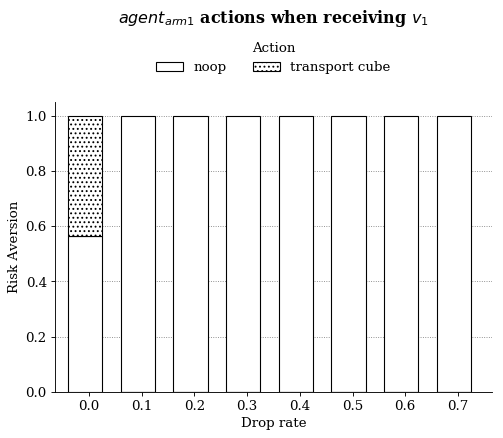
\includegraphics[width=0.5\textwidth]{imgs/exp-3-2msg-grounding-a1.png}
\caption[Reaction to received communication relative to the drop rate]{Reaction to received communication relative to the drop rate.}
\label{fig:exp-3-grounding}
\end{figure}

As shown in table~\ref{tab:exp-3-assigments}, by putting a prerequisite usage of message $0$, the number of possible valid protocols is reduced.  As expected, due to this reduction, the number of optimal solutions is lower. Also, no optimal solutions are found when the drop rate is too high (fig~\ref{fig:exp-3-behaviour}).
\begin{table}[ht]
    \centering
    \begin{tabular}{lrr}
    \toprule
    $\abs{V} $ & \multicolumn{2}{c}{Valid assignment} \\
    \midrule
    $2$ & 6.2\% & (1/16)\\
    $3$ & 14.0 & (9/64) \\
    $4$ & 19.1\% & (49/256)\\
    $8$ & 27.5\% & (16129/58466)\\
    \bottomrule
    \end{tabular}
    \caption[Valid vocabulary assignments with unreliable channel]{Valid vocabulary assignments when channel is unreliable. This channel requires the $v_0$ to convey intent $00$.}
    \label{tab:exp-3-assigments}
\end{table}


\begin{figure}[ht]
\centering
\begin{minipage}[t]{.5\textwidth}
    \centering
    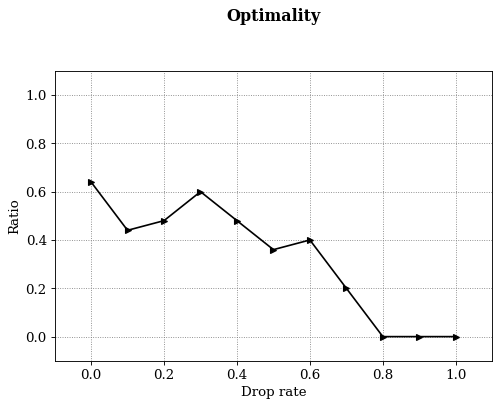
\includegraphics[width=0.95\textwidth]{imgs/exp-3-2msg-optimality.png}
    \caption[Optimality relative to the drop rate]{Optimality of learning relative to the drop rate.}
    \label{fig:exp-3-behaviour}
\end{minipage}%
% \begin{minipage}[t]{.50\textwidth}
%     \centering
%     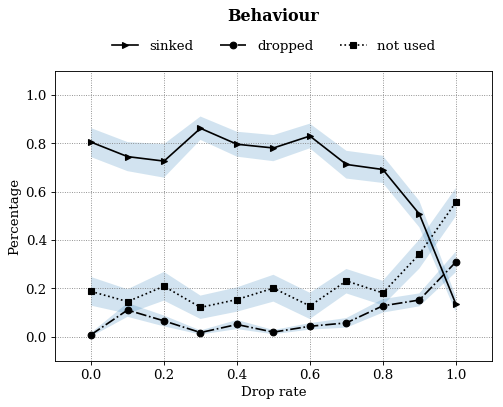
\includegraphics[width=0.95\textwidth]{imgs/exp-3-2msg-behaviour.png}
%     \caption[Behaviour of agents relative to the drop rate]{Behaviour of agents relative to the drop rate.}
%     \label{fig:protocol-4msg-good}
% \end{minipage}
\end{figure}


% %%%%%%%%%%%%%%%%%%%%%%%%%%%%%%%%%%%%%%%%%%%%%%%%%%%%%%
% %%%%%%%%%%%%%%%%%%%%%%%%%%%%%%%%%%%%%%%%%%%%%%%%%%%%%%
% %%%%%%%%%%%%%%%%%%%%%%%%%%%%%%%%%%%%%%%%%%%%%%%%%%%%%%
% %%%%%%%%%%%%%%%%%%%%%%%%%%%%%%%%%%%%%%%%%%%%%%%%%%%%%%

\section{Fully agent controlled}

Finally, the constraint that the agent controlling $arm3$ is scripted can be relaxed. Table~\ref{tab:3c-opti} shows that the scenario used can also be solved using fully decentralised learning with each arm being controlled by a learning agent. 

\begin{table}[ht]
\centering
    \begin{tabular}{lrr}
    \toprule
    Measurement &  $\abs{V} = 2$ & $\abs{V} = 4$ \\
    \midrule
    Optimality & $0.86$ & $0.96$\\
    \midrule
    Sinked (\%) &  $96.37 \pm 12.48$ & $98.83 \pm 7.80$ \\
    Dropped (\%) &  $1.62 \pm  6.84$  & $7.66 \pm 1.01$\\
    Not used (\%) & $2.01 \pm 10.75$ & $1.59 \pm 0.15$ \\
    \bottomrule
    \end{tabular}
    \caption[Optimality and behaviour with fully decentralised learning]{Optimality and behaviour when control is leanrned in a fully decentralised fashion.}
    \label{tab:3c-opti}
\end{table}


    
% Why 2 messages => 
% - setting with only two different possible protocol 
% - can not have a suboptimal usage of the channel. It is either used correctly and provide a optimal solution or not and then solution is suboptimal. The channel is thus used at its maximum complexity. With $\abs{V} =2$, only two valid protocol exists, 
% # Conclusion
% - Set rwdc to -0.1 to keep setting rationa

% # Conclusion
% - Cost of communication can be used to help the grounding of communication
%     - Must be careful not to be too drastic with the cost
%     - having no cost of communication let the agent decide fully the meaning of the sent message. This result is a slightly higher ratio of optimal solution indeed, their is no guidance compared to a small communication reward
        
% - Reward influence grounding of communication % Discussion
\chapter{Future Work and Conclusion}
\lhead{\emph{Conclusion}} 
\label{chap:conclusion}

\section{Future research}

Several lines of research arising from this work should be pursued. Firstly, investigating more complex problems and learning methods might prove important. The current work relies solely on tabular Q-Learning and might be too limited for learning more complex tasks. Also, future research is needed to investigate the possibilities of using delayed instead of instantaneous communication. Finally, in the current work, the agents have no implicit incentive to be fast. It is thus possible to assume that the influence of the discount rate on the quality of the protocols might change when the incentive exists. This assumption should be addressed in future studies.

\section{Conclusion}

This work demonstrates that a simulated transport problem involving robotic arms can be solved using decentralised learners and inter-agent communication. Being able to solve a reinforcement learning problem in a decentralised manner can help when the problem becomes intractable by a centralised scheme. Furthermore, this work shows that increasing the vocabulary size available to a communicating agent improves the quality of the learned solution. On a higher level, the cost of communication can be used to influence the grounding of communication used by the agents. When a problem can be aliased to a referential game, a low discount rate can be used to increase the chance of converging to an ideal protocol.


 % Conclusion


% ----------------------------------------------------------------
% Now begin the Appendices, including them as separate files

\addtocontents{toc}{\vspace{2em}} % Add a gap in the Contents, for aesthetics

\appendix % Cue to tell LaTeX that the following 'chapters' are Appendices
\chapter{Determination of the grounding of the protocol}
\lhead{\emph{Appendices}} 
\label{app:grounding}	

The grounding of the communication is required when the protocol needs to be analysed. The determination of the grounding is done in 3 steps. In the first one, the interpretation given to each symbol of the vocabulary is determined. Then, the intent conveyed by each symbol is looked at. Finally, the information gained by the two preceding steps is merged to get the final grounding. Before looking at the grounding of the communication, the learned agents must be evaluated. Only protocol leading to an optimal solution are of interest. Afterwards, the greedy policy is determined by looking at the Q-estimate of each agent.

The following presents how the grounding is found. The example is taken from a training sessions with parameters $r_{com} = -0.1$, $r_{time} = -0.1$,  and $\gamma = 0.9$.

\paragraph*{Interpretations of the symbols}
The interpretation of the symbols by the feeding arms $agent_{arm1}$ and $agent_{arm2}$ is looked at first. In order to determine the interpretation, it is sufficient to look at what action the agent takes relative to the message received. Thus, only the states in which the agents could potentially transport a cube are of interest. If the agent decides to transport a cube, the message has been interpreted as "safe for me" and "not safe for me" otherwise. It is then possible to construct a table of interpretation and the right part of the protocol graph (tab.~\ref{tab:grounding-inter}, fig.~\ref{fig:grounding-inter}). 

\begin{table}[H]
\centering
\begin{minipage}[b]{.5\textwidth}
\vspace{0pt}
     \centering
    \begin{tabular}{lll}
    \toprule
    Symbol & $agent_{arm1}$ & $agent_{arm2}$ \\
    \midrule
    $v_0$ & not safe & not safe \\
    $v_1$ & not safe &  safe \\
    $v_2$ & not safe & not safe \\
    $v_3$ & safe & safe \\
    \bottomrule
    \end{tabular}
    \caption[Interpretation of symbols by the feeding agents]{Example of an interpretation of symbols by $agent_{arm1}$ and $agent_{arm2}$.}
    \label{tab:grounding-inter}
\end{minipage}%
\begin{minipage}[b]{.50\textwidth}
    \vspace{0pt}
    \centering
    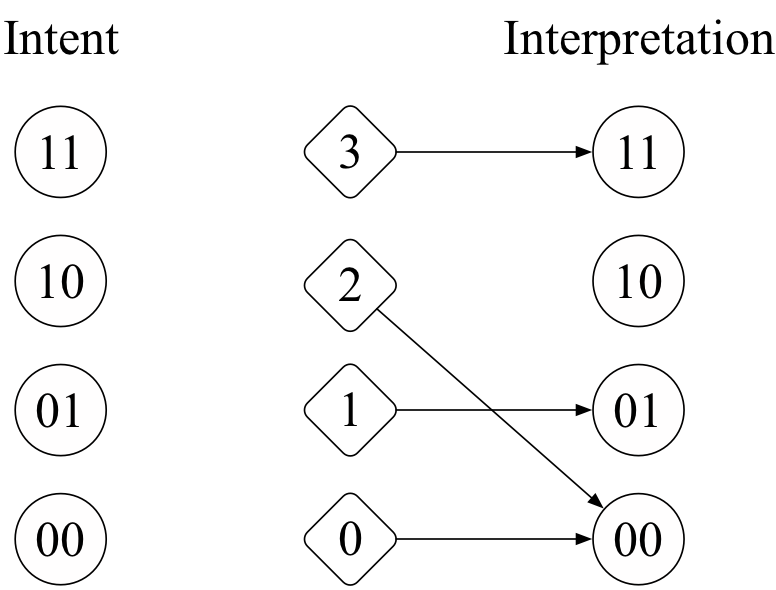
\includegraphics[width=0.75\textwidth]{imgs/grounding-inter.png}
    \caption[Protocol graph related to the interpretation of symbols by the feeding agents]{Protocol graph related to the interpretation of symbols by the feeding agents as shown in tab.~\ref{tab:grounding-inter}.}
    \label{fig:grounding-inter}
\end{minipage}
\end{table}

It is also possible to represent the assignment of the symbols using a set notation. This notation is useful when the grounding process needs to be implemented programmatically (tab.~\ref{tab:grounding-set-inter}).

\begin{table}[H]
\centering
\begin{minipage}[b]{.5\textwidth}
\vspace{0pt}
    \centering
    \begin{tabular}{lll}
    interpretation-$11$ & = & $\{v_3\}$ \\
    interpretation-$10$ & = & $\{\emptyset\}$ \\
    interpretation-$01$ & = & $\{v_1\}$\\
    interpretation-$00$ & = & $\{v_0, v_2\}$\\
    \end{tabular}
    \caption{Vocabulary assignment related to the interpretation.}
    \label{tab:grounding-set-inter}
\end{minipage}%
\begin{minipage}[b]{.50\textwidth}
    \vspace{0pt}
    \centering
    \begin{tabular}{lll}
    intent-$11$ & = & $\{v_1, v_3\}$ \\
    intent-$10$ & = & $\{v_2, v_0\}$ \\
    intent-$01$ & = & $\{v_1, v_2\}$\\
    intent-$00$ & = & $\{v_0, v_2\}$\\
    \end{tabular}
    \caption{Vocabulary assignment related to the intent.}
    \label{tab:grounding-set-intent}
\end{minipage}
\end{table}


\paragraph*{Intents of the symbols}
The intent transmitted by each symbol is then looked at. For this, the Q-table of $agent_{arm3c}$ is used. By looking at each sub state (see table~\ref{tab:agent3c-substate}), the sets containing the symbols relative to each intent can be constructed. Continuing with the same example, the sets presented in table~\ref{tab:grounding-set-intent} can be constructed. Based on this table, the protocol graph can then be completed (fig.~\ref{fig:grounding-intent}).

\begin{figure}[H]
    \vspace{0pt}
    \centering
    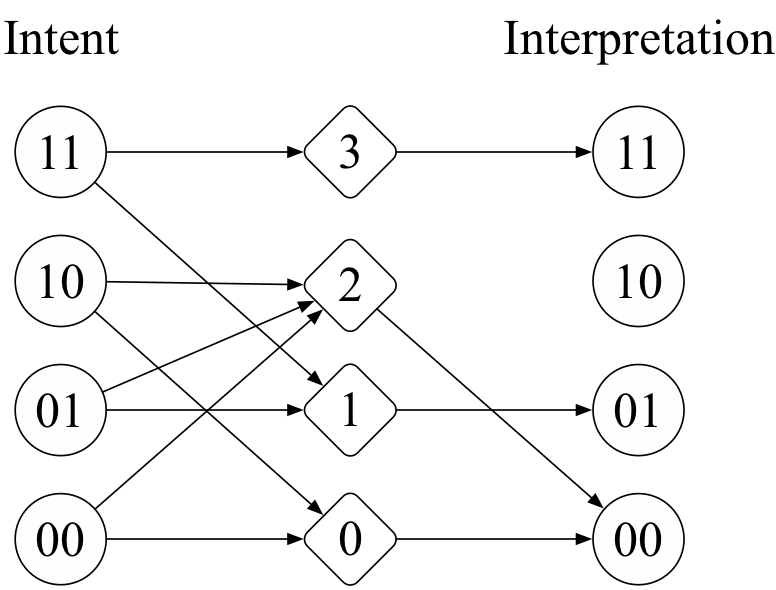
\includegraphics[width=0.375\textwidth]{imgs/grounding-intent.png}
    \caption[Protocol graph related to the intent of the symbols]{Protocol graph related to the intent transmitted by the symbols by the receiving agent.}
    \label{fig:grounding-intent}
\end{figure}

\paragraph*{Grounding of the protocol}

Finally, based on the sets in tables~\ref{tab:grounding-set-inter}~and~\ref{tab:grounding-set-intent}, it is possible to determine the final grounding of the communication. Table~\ref{tab:grounding-grounding} shows the final results for the example. The constructed sets enable the creation of the protocol graph depicting which intent is correctly transmitted through the channel (fig.~\ref{fig:grounding-final}).

\begin{table}[ht]
    \centering
    \begin{tabular}{lllll}
    grounding-$11$ & $=$ & intent-$11$ $\cap$ interpretation-$11$ & $= \{v_3\}$ \\ 
    grounding-$10$ & $=$ & intent-$10$ $\cap$ interpretation-$10$ & $= \{\emptyset\}$ \\ 
    grounding-$01$ & $=$ & intent-$01$ $\cap$ interpretation-$01$ & $= \{v_1\}$ \\ 
    grounding-$00$ & $=$ & intent-$00$ & $= \{v_0, v_2\}$ \\ 
    \end{tabular}
    \caption{Vocabulary assignment related to the grounding.}
    \label{tab:grounding-grounding}
\end{table}

\begin{figure}[H]
    \vspace{0pt}
    \centering
    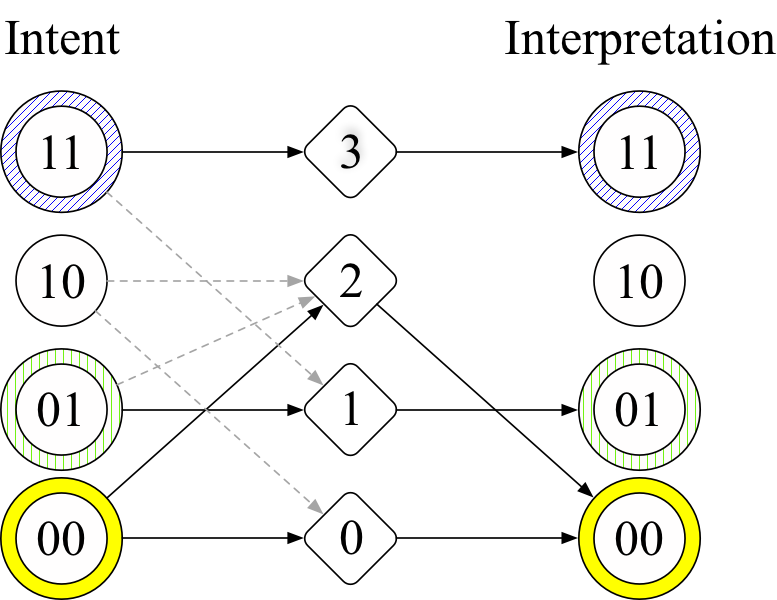
\includegraphics[width=0.375\textwidth]{imgs/grounding-final.png}
    \caption{Final protocol graph related to the example.}
    \label{fig:grounding-final}
\end{figure}

The protocol type of the example is thus $1011$. This learned protocol is non-ideal even though it leads to an optimal solution.

\chapter{Architecture overview}
\lhead{\emph{Appendices}} 
\label{app:arch-overview}	

The learning environment used during the experiments is inspired by the OpenAI multi-agent environment \cite{lowe_multi-agent_2017}. The simulation can be separated into distinct parts. The \textit{world} is the abstract concept where the agents will interact with each other. The second part of the architecture is involved into the reinforcement learning process. It is separated into \textit{scenarios} and \textit{runners}. Figure~\ref{fig:architecture-overview} depicts the overall architecture. The scenarios act as an interface between the world and the runners while the latter is used to manage the necessary process for the reinforcement learning. In order to simulate the interaction between entities, discrete time steps are used. For clarity, the following assumes that cubes are being transported.

\begin{figure}[h!]
\centering
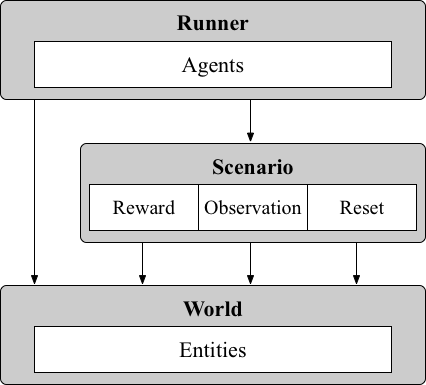
\includegraphics[width=0.5\textwidth]{imgs/architecture-overview.png}
\caption[Overview of the experiment architecture]{Overview of the experiment architecture}
\label{fig:architecture-overview}
\end{figure}

\section{World}

The world is the sandbox in which all \textit{entities} involved in an experiment will interact. Three different representations of physical objects were used. The internal state of all entities can be queried to enable the creation of the observation required by the agents. Entities can be separated into two classes. After being created, \textbf{scripted} entities will react to the changes in the environment automatically while \textbf{dynamic} entities are controlled by an external process. Dynamic entities are linked to a learning agent that will decide on the next action.   

\subsection{Buffer}
\label{sec:archi-uffer}
The buffer can be seen as a wrapper around a FIFO queue. It is the equivalent to a crate where cubes can be stocked. The size of the buffer can be limited or infinite. When there is no space left in the queue, any new element added to it will be considered lost (i.e. dropped) for the remaining of the episode.

\subsection*{Available endpoints to other entities}
\begin{enumerate}[label=(\arabic*)]
\item \textbf{get}: If a cube is available in the buffer, takes it out and returns it.
\item \textbf{put}: If space is available in the queue, puts the given cube in the buffer. Drops it otherwise.
\end{enumerate} 

\subsection*{Available state information}
\begin{itemize}[noitemsep]
\item Buffer full status (boolean)
\item Buffer empty status (boolean)
\item Current size of the queue (integer)
\item Maximum size of the queue (integer)
\end{itemize}

\subsection{Conveyor}

A conveyor acts as an automatic non-instantaneous transporter of cubes between two different points. In a nutshell, a cube placed at one end of the conveyor (\textit{head}) will be available at the other end (\textit{tail}) after a delay $t$. The head and tail of the conveyor are also buffers as described in section~\ref{sec:archi-uffer}.

The conveyor is automatic in the sense that as soon as its head buffer is full, it will start the transfer. It is assumed that the head buffer is moving along the conveyor making it unavailable for deposit during the transportation. After $t$ time steps have elapsed, the content of the head buffer will have been transferred to the tail buffer. As for a normal buffer, any cube not fitting in the tail buffer will be dropped. Similarly to the buffer entity, two endpoints are available.

\subsection*{Available endpoints to other entities}
\begin{enumerate}[label=(\arabic*)]
\item \textbf{get}: If a cube is available in the tail buffer, takes it out and returns it.
\item \textbf{put}: If space is available in the head buffer and the conveyor is not moving, puts the given cube in the buffer. Drops it otherwise.
\end{enumerate} 

\subsection*{Available state information}
\begin{itemize}[noitemsep]
\item Speed $t$ of the conveyor (integer)
\item Position of the conveyor (integer)
\item Buffer information for head buffer
\item Buffer information for tail buffer
\end{itemize}


\subsection{Robotic Arm}

The interaction with a robotic arm is done via two different controllers depicted in figure~\ref{fig:architecture-arm-controller}. The \textit{physical controller} provide a low-level API. The available endpoints in the low-level API are abstractions of the atomic actions a robotic arm can do. Such action can be moving to point $A$, gripping, releasing, etc. for example. For a more in-depth look at the physical controller, see \ref{app:ros-overview}. The low-level API is then leveraged by a \textit{meta controller} to provide high-level actions endpoints. The meta controller combines low-level actions into higher-level actions such as transporting an object from point $A$ to point $B$. In order to populate the high-level API, it is assumed that the possible pickup and deposit positions are fixed and known in advance.

\begin{figure}[H]
\centering
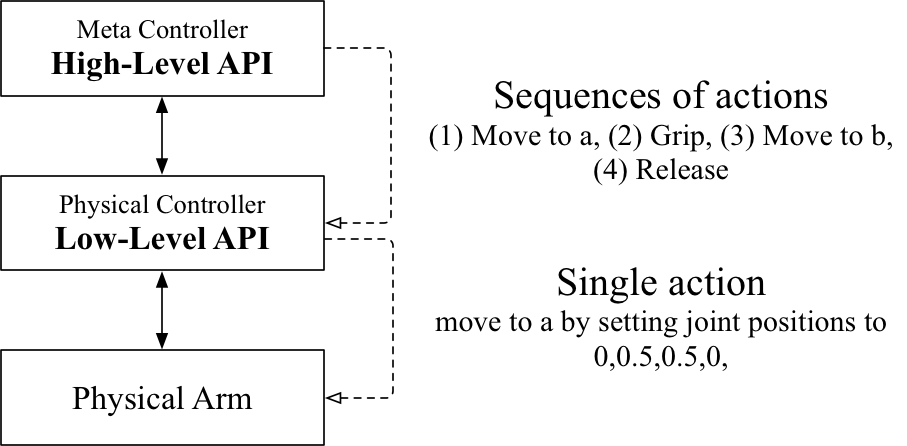
\includegraphics[width=0.7\textwidth]{imgs/ros-gazebo-archi-1.png}
\caption[Overview of the architecture used to control the robotic arms]{Overview of the architecture used to control the robotic arms}
\label{fig:architecture-arm-controller}
\end{figure}


\subsection*{Available endpoints to higher level}
\begin{enumerate}[label=(\arabic*)]
\item \textbf{$move_{p_i, d_j}$} provides endpoints to transport a cube from any pickup position $p_i$ to any deposit position $d_i$.
\item \textbf{noop} indicates to the physical controller that no action should be taken.
\end{enumerate} 

\subsection*{Available state information}
\begin{itemize}[noitemsep]
\item High-level action taken at the last time step.
\item Busy status (indicate if an low-level action is being realised)
\item Number of possible actions
\end{itemize}

\section{Scenarios \& Runners}

A scenario provides a view of the underlying world specifically tailored to the need of a reinforcement learning experiment. It creates the reward and the observation vector for each agent involved. One other duty of the scenario is to reset the world into a predefined state.

Each training session is managed by a runner. The role of the runner is to orchestrate and manage the learning. It will provide the necessary observation to the agents for their decision and update process. The runner is also in charge of indicating to the world which action should be realised in the next time step.  

\subsection{Learning Cycle}

The learning is separated into episodes. An episode can terminate either when the defined scenario is considered solved (example. no cube left to transport) or when a predefined number of steps have been done. The world is reset after each episode. The created framework is general and applies the following learning cycle.

\subsection*{Initialisation}

\begin{enumerate}[noitemsep,topsep=0pt,parsep=0pt,partopsep=0pt,label=(\arabic*)]
\item \textbf{Create the world} by creating the involved entities (buffers, conveyors, arms, etc.) as well as their relationship. Only done once per training session.
\item \textbf{Reset the world} into an initial state (ready for training). This step is repeated before each episode.
\end{enumerate}

\subsection*{Training}

The training process is managed at the runner level. The current implementation assumes that all actions and all environment changes resulting from those actions have been performed before the world moves to the next time step. 

\begin{enumerate}[noitemsep,topsep=0pt,parsep=0pt,partopsep=0pt,label=(\arabic*)]
\item \textbf{Get observation}: Get $o_t^{a_i}$ for every agent $a_i$ by querying the scenario.
\item \textbf{Action selection}: Each agent selects his action based on $o_t^{a_i}$.
\item \textbf{Apply selected action}: The selected actions are applied and all entities states are updated accordingly.
\item \textbf{Get feedback from the environment}: Based on the outcome of the actions, reward signal and next observations are constructed by the scenario.
\item If the task is considered solved (ex: no object left to transport in the system), the episode terminates. Otherwise go back to 1
\end{enumerate}


\chapter{Robotic arm Python wrapper}
\lhead{\emph{Appendices}} 
\label{app:ros-overview}	
Due to time restriction, the interactions with the physical simulator or the real arms have not been implemented. Despite this, the outline of the physical controller is detailed below for future reference.

\section{Robotic interface}

The Robot Operation System (ROS) provides a software framework to help developers create software involving robots. It includes several open source libraries and tools (BSD license) to "encourage collaborative robotics software development" by providing useful abstraction over hardware, drivers, etc. Since its inception in 2007, ROS has been used to interface with a wide range of robots. Due to the collaborative approach taken by the ROS developers, hundreds of libraries as well as robotic interface have been contributed to the ROS eco-system \cite{noauthor_robot_2017}. This in turn enables developers to concentrate on innovation by building on each other's work. 

ROS is a distributed framework of processes (referred as Nodes in the documentation) performing tasks. The framework is designed to be loosely coupled where each node is supposed to be responsible for a single task. 

The communication between nodes is based on a publish-subscribe pattern using named logical channels called topics. Each node can then send message or receive message by either publishing or subscribing to a topic. ROS also provides services to cope with the need of remote procedure call (RPC) request / reply interactions. The communication protocol is defined by a pair of messages (request and reply). In order for the different node to find each other, ROS provides a Master nodes responsible for the registration as well as the look-up of topics \cite{noauthor_master_nodate}. After successful registration and look-up, the nodes communicate peer-to-peer by publishing a message to a topic or by sending a message to a service. A message is a simple data structure composed of typed fields.

Gazebo provides an open source robot simulation environment. It provides a wide range of tool to help software developers to easily design, test, improve algorithms or robots in realistic scenarios. Gazebo can directly and easily interface with ROS in place of the actual physical robot.

\subsection{Robotic arm}

The physical robotic arm selected was the PhantomX Pincher Robot Mark II \cite{noauthor_phantomx_nodate} or commonly referred as the Turtlebot arm. This arm provides 4 degrees-of-freedom as well as pinching. A model of the arm is available both for ROS and Gazebo. 

\section{Architecture design}

The goal of the physical controller is to abstract and encapsulate the possible action of the different robotic arms.

\subsection{Overview}

\begin{figure}
\centering
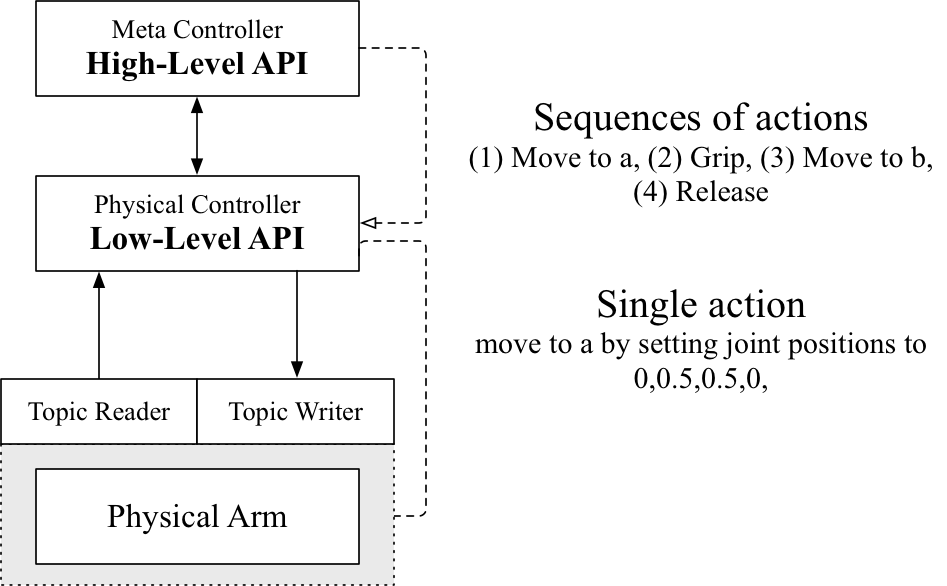
\includegraphics[width=0.7\textwidth]{imgs/ros-gazebo-archi.png}
\caption[Overview of the ROS wrapper architecture]{Overview of the software architecture layers. The greyed items are only here for comprehension purposes and are not part of the physical controller.}
\label{fig:ros-wrapper-architecture}
\end{figure}

Figure ~\ref{fig:ros-wrapper-architecture} shows the different level of abstraction implemented. The interface level provides two abstracted access points to ROS. A topic reader provides access to the latest message published in the topic enable the higher level to know the state of the arm while a topic writer enables the publication of a message to alter the state.

\begin{figure}

\tikzset{
    decision/.style={diamond, draw, fill=blue!20, text width=4.5em, text badly centered, node distance=3cm, inner sep=0pt},
    block/.style={rectangle, draw, fill=blue!20, text width=5em, text centered, rounded corners, minimum height=4em},
    line/.style={draw, -latex'},
    cloud/.style={draw, ellipse,fill=red!20, node distance=3cm, minimum height=2em}
}

\centering
\begin{tikzpicture}[node distance = 2cm, auto]
    % Place nodes
    \node [cloud] (init) {Apply joint position};
    \node [block, below of=init] (apply) {Apply new joint values};
    \node [decision, below= 1cm of apply] (decide1) {reach joint position?};
    \node [decision, below= 1cm of decide1] (decide2) {timeout?};
    \node [cloud, right=1.5cm of decide1] (end) {end};
    \node[left=1.5cm of decide1, scale=0.05](inv){};
    
    % % Draw edges
    \path [line] (init) -- (apply);
    \path [line] (apply) -- node {wait $t$ s} (decide1);
    \path [line] (decide1) -- node {yes}(end);
    \path [line] (decide1) -- node {no}(decide2);
    \path [line] (decide2) -| node[below]{yes}(end);
    
    \path[-,draw] (decide2) -| node[below]{no} (inv.south);
    \path[line]{} (inv.south) |- node{} (apply);
\end{tikzpicture}

\caption[Overview of a controller work-flow]{Example of work-flow abstracted by the arm controller. For the user, after applying a new set of joint position, the controller will either return a zero or non-zero exit status depending on the result of the interaction with the "physical" arm. A non-zero exit code could be returned if a user breaks the arm by applying malicious values.}
\label{fig:ros-controller-process}
\end{figure}


The two interfaces are used to create the physical controller. The goal of the controller is to provide a simple low-level API to interact with the underlying physical object (either real or simulated). The controller abstracts all the steps taken in order to execute an action or raise an exception in case of an error. Figure ~\ref{fig:ros-controller-process} shows the abstracted process for applying new joint angles to the arm. Resting on this process and knowing the joint-position needed to reach point $A$, it is then possible to create a "move to point $A$" endpoints. The architecture leaves the error handling to the user. 

%OpenAI gym framework [REF] is used as a base for the interaction with the environment. It provides a well defined and proved framework for reinforcement learning. Several scenarios have been implemented to enable research with different observation spaces (cameras instead of joint angles, known position of the cube, etc.). It is at the environment level that the exception and failure are currently handled (i.e. reset the arm is case of breakage, etc.).

%\subsection{Limitations}

%Currently the implementation is not capable of the gripping action. Also the robotic arm joints are using the PositionJointInterface [REF] instead of the EffortJointInterface [REF] to simplify the implementation.

%\input{Appendices/AppendixC} % Appendix Title

\addtocontents{toc}{\vspace{2em}} % Add a gap in the Contents, for aesthetics
\backmatter

%% ----------------------------------------------------------------
\label{Bibliography}
\lhead{\emph{Bibliography}} % Change the left side page header to "Bibliography"
\printbibliography
%\bibliographystyle{unsrt} % Use the "unsrtnat" BibTeX style for formatting the Bibliography
%\bibliography{Bibliography} % The references (bibliography) information are stored in the file named "Bibliography.bib"

\end{document} % The End
%% ----------------------------------------------------------------